\documentclass[12pt,a4paper,twoside]{article}

%%% Packages %%%
\renewcommand{\baselinestretch}{1.0} % Change to 1.65 for double spacing

% text area 15.5cm x 23.7cm
\usepackage[a4paper,top=3.0cm,bottom=3.0cm,left=3.0cm,right=2.5cm]{geometry}

%\usepackage{natbib}

%\usepackage{acro}
\usepackage[acronym,section=section]{glossaries}
\usepackage{caption}
\usepackage{subcaption}

\usepackage{afterpage}
\usepackage{mathrsfs,amsmath,amsfonts,amssymb}
\usepackage{array}
\usepackage[main=czech, english,german,french,greek]{babel}
\usepackage{booktabs}
%\usepackage[small,bf]{caption}
\usepackage{color}
\usepackage{colortbl} % rows and columns to be colored
\usepackage{enumitem}
\usepackage{fancyhdr} % extensive facilities, both for headers and footers
\usepackage[T1]{fontenc}
\usepackage{gensymb} % symbols
\usepackage{graphicx} % \includegraphics
\usepackage{here}
\usepackage[colorlinks=true,urlcolor=blue,filecolor=black,linkcolor=black,citecolor=black]{hyperref}
\usepackage[utf8]{inputenc}
\usepackage{lmodern} % fonts in a LaTeX document
\usepackage{multirow}
\usepackage{pdflscape} % allows to introduce a landscape page in the document
\usepackage{pdfpages} % allows to include external PDF pages
%\usepackage{subfigure} % subplot
\usepackage{textcomp} % many text symbols
\usepackage{tikz} % tikz image
\usetikzlibrary{shapes,trees}
\usepackage{varioref} % reference "on page #" \vref \vpageref
\usepackage{wasysym} % provides many symbol e.g. male, female, astronomical symbols
\usepackage{wrapfig}

%%%Colored source codes
\usepackage{listings}
\definecolor{mygreen}{rgb}{0,0.6,0}
\definecolor{mygray}{rgb}{0.5,0.5,0.5}
\definecolor{mymauve}{rgb}{0.58,0,0.82}
\definecolor{ashgrey}{rgb}{0.7, 0.75, 0.71}

\lstset{
  backgroundcolor=\color{white},   % choose the background color; you must add \usepackage{color} or \usepackage{xcolor}; should come as last argument
  basicstyle=\footnotesize,        % the size of the fonts that are used for the code
  breakatwhitespace=false,         % sets if automatic breaks should only happen at whitespace
  breaklines=true,                 % sets automatic line breaking
  captionpos=b,                    % sets the caption-position to bottom
  commentstyle=\color{mygreen},    % comment style
  deletekeywords={...},            % if you want to delete keywords from the given language
  escapeinside={\%*}{*)},          % if you want to add LaTeX within your code
  extendedchars=true,              % lets you use non-ASCII characters; for 8-bits encodings only, does not work with UTF-8
  firstnumber=1000,                % start line enumeration with line 1000
  frame=single,	                   % adds a frame around the code
  keepspaces=true,                 % keeps spaces in text, useful for keeping indentation of code (possibly needs columns=flexible)
  keywordstyle=\color{blue},       % keyword style
  language=C,                 % the language of the code
  morekeywords={*,...},            % if you want to add more keywords to the set
  numbers=left,                    % where to put the line-numbers; possible values are (none, left, right)
  numbersep=5pt,                   % how far the line-numbers are from the code
  numberstyle=\tiny\color{mygray}, % the style that is used for the line-numbers
  rulecolor=\color{black},         % if not set, the frame-color may be changed on line-breaks within not-black text (e.g. comments (green here))
  showspaces=false,                % show spaces everywhere adding particular underscores; it overrides 'showstringspaces'
  showstringspaces=false,          % underline spaces within strings only
  showtabs=false,                  % show tabs within strings adding particular underscores
  stepnumber=2,                    % the step between two line-numbers. If it's 1, each line will be numbered
  stringstyle=\color{mymauve},     % string literal style
  tabsize=2,	                   % sets default tabsize to 2 spaces
  title=\lstname                   % show the filename of files included with \lstinputlisting; also try caption instead of title
}

%% language C colored
\lstdefinestyle{customc}{
  belowcaptionskip=1\baselineskip,
  breaklines=true,
  frame=N,
  xleftmargin=\parindent,
  language=C,
  showstringspaces=false,
  basicstyle=\footnotesize\ttfamily,
  keywordstyle=\bfseries\color{green!40!black},
  commentstyle=\itshape\color{purple!40!black},
  identifierstyle=\color{blue},
  stringstyle=\color{orange},
    breakatwhitespace=false,
    captionpos=b,
    keepspaces=true,
    numbers=left,
    numbersep=5pt,
    showspaces=false,
    showstringspaces=false,
    showtabs=false,
    tabsize=2,
}

\lstdefinestyle{customc_config}{
  belowcaptionskip=1\baselineskip,
  breaklines=true,
  frame=single,
  xleftmargin=0pt,
  language=C,
  showstringspaces=false,
  basicstyle=\footnotesize\ttfamily,
  keywordstyle=\bfseries\color{green!40!black},
  commentstyle=\itshape\color{purple!40!black},
  identifierstyle=\color{blue},
  stringstyle=\color{orange},
    breakatwhitespace=false,
    captionpos=b,
    keepspaces=true,
    numbers=none,
   	numbersep=0pt,
    showspaces=false,
    showstringspaces=false,
    showtabs=false,
    tabsize=2,
}


\parskip = 4pt	% space between paragraphs

%% apendixy
\usepackage{pdfpages}


% \renewcommand{\thefigure}{\thesection.\arabic{figure}}
% \renewcommand{\thetable}{\thesection.\arabic{table}}
% \renewcommand{\theequation}{\thesection.\arabic{equation}}

\newcommand{\blankpage}{
\newpage
\thispagestyle{empty}
\mbox{}
\newpage
}

%% Today format month, year
\newcommand{\todayMonthYear}{
\ifcase \month \or Leden\or Únor\or Březen\or %
Duben\or Květen \or Červen\or Červenec\or Srpen\or Září\or Říjen\or Listopad\or %
Prosinec\fi \ \number \year
}

\newcommand{\inProgress}{\textbf{\color{red} \Large Rozpracováno, nepublikováno !!!}}

\newcommand{\notFinished}{\textbf{\color{orange} \Large Nedokončeno, doplnit !!!}}

%%Uvodni stranka
\definecolor{cvutcolor}{cmyk}{1, 0.43, 0, 0} %modra CVUT
\newlength{\titlewidth}
\setlength{\titlewidth}{\textwidth}
\addtolength{\titlewidth}{-1.7cm}
\newlength{\heightofhw}

\newcommand{\TitlePage}[3]{{
	\thispagestyle{empty}
	\parbox{0.7cm}{\color{cvutcolor}\rule{0.35cm}{\textheight}}
	{\parbox[0][\textheight][t]{\titlewidth}{
		\sffamily
		%\vspace{1pt}
		
\includegraphics[height=4.1cm]{img/logo_CVUT.pdf}\\[0.5em]
		%\put(10,40){\parbox{8cm}{\Large  \textbf{České}\\[0.3em] \textbf{vysoké učení}\\[0.3em] \textbf{technické}\\[0.3em] \textbf{v Praze}\\[.6em]}} \\[.1em]
		\textbf{\Large
			\color{cvutcolor} Fakulta Elektrotechnická \\[0.3em]
			\color{black} Katedra radioelektroniky
		}\\[6em]
		\color{black}{\Large \textbf{Bakalářská práce}}\\[0.8em]
		{\huge \textbf{#2}}\\[0.8em]
		{\Large \textbf{#3}}\\[0.8em]
		
		\vspace*{1.5cm}
		\color{cvutcolor}{\Large \textbf{#1}}\\[0.8em]

		\vspace*{1cm}
		~\vfill


		\textbf{\large
			\color{black} Vedoucí práce:
		\color{cvutcolor} Ing. Stanislav Vítek, Ph.D.
		}\\[0.2cm]
		\textbf{\large
 			\color{black} Studijní program:
 			\color{cvutcolor}  Elektronika a komunikace
		}\\[0.2cm]
		\textbf{\Large \color{black} Praha, \todayMonthYear}
		\vspace{2pt}
	}}
	\newpage
}}




% \begin{titlepage}
% \pagestyle{empty}

% \begin{minipage}{95mm}
% 	\vspace{1mm}
% 	\includegraphics[height=20mm]{images/logo_mmtg.pdf}\\
% 	\textsc{\scriptsize Department of Radioelectronics}\\
% \end{minipage}
% \begin{minipage}{60mm}
% 	\includegraphics[height=21mm]{images/logo_fee.pdf}\\
% 	\textsc{\scriptsize Doctoral program in Radioelectronics}\\
% \end{minipage}\\ [2cm]

% \hspace{1cm}\LARGE\textsc{Doctoral Thesis Proposal}\\\vspace{10mm}
% \hspace{5mm}{\color{cvut}\rule{15cm}{1mm}}\\\vspace{10mm}
% \hspace{1cm}\parbox[c][2.5cm][c]{13cm}{\Huge\textbf{EMCCD camera image processing}}\\\vspace{15mm}
% \hspace{5mm}{\color{cvut}\rule{15cm}{1mm}}

% \vspace{2cm}\hspace{1cm}
% \LARGE\textsc{Maria Nasyrova}

% \vspace{2cm}\hspace{1cm}
% \begin{minipage}{10cm}
% 	\LARGE
% 	Thesis supervisor
% 	\newline Ing. Stanislav V{í}tek, Ph.D.
% 	\newline CTU in Prague
% \end{minipage}

% \vfill\hspace{1cm}
% \LARGE Prague, September 2018

% \newpage

% \vspace*{1cm}

% \begin{tabular}{ll}
% \large \textbf{Applicant} & \large Ing. Maria Nasyrova\\
% \large  & \large Czech Technical University in Prague\\
% \large  & \large Faculty of Electrical Engineering\\
% \large  & \large Department of Radioelectronics\\
% \large  & \large Technická 2\\
% \large  & \large 166 27, Praha 6\\
% \large  & \large office: +420 224 352 113\\
% \large  & \large email:	 nasyrmar@fel.cvut.cz\\
% \large  & \large \\
% \large  & \large \\
% \large \textbf{Thesis supervisor} & \large Ing. Stanislav V{í}tek, Ph.D.\\
% \large  & \large Czech Technical University in Prague\\
% \large  & \large Faculty of Electrical Engineering\\
% \large  & \large Department of Radioelectronics\\
% \large  & \large Technická 2\\
% \large  & \large 166 27, Praha 6\\
% \large  & \large office: +420 224 352 226\\
% \large  & \large \\
% \large  & \large \\
% \large  & \large \\

% \end{tabular}

% \end{titlepage}

\newcommand{\Author}{Jan Závorka}
\newcommand{\Title}{Interaktivní hra využívající \\ [.2em] IoT prostředky}
\newcommand{\TitleEN}{Interactive Game Based on IoT Technology}

%\renewcommand*{\glossaryentrynumbers}[1]{}

\newacronym{maia}{MAIA}{Meteor Automatic Imager and Analyze}
\newacronym{ccd}{CCD}{charge-coupled device}
\newacronym{spmn}{SPMN}{SPanish Meteor Nerwork}
\newacronym{cams}{CAMS}{Cameras for Allsky Meteor Surveillance}
\newacronym{cmn}{CMN}{Croatian Meteor Network}
\newacronym{pfn}{PFN}{Polish Fireball Network}
\newacronym{camo}{CAMO}{Canadian Automated Meteor Observatory}
\newacronym{mcp}{MCP}{microchannel plate}
\newacronym{emccd}{EMCCD}{electron multiplying CCD}
\newacronym{cmos}{CMOS}{Complementary Metal–Oxide–Semiconductor}
\newacronym{ebi}{EBI}{Equivalent  Background  Illumination}
\newacronym{snr}{SNR}{signal-to-noise ratio}
\newacronym{psf}{PSF}{point spread function}
\newacronym{fwhm}{FWHM}{full width at half maximum}
\newacronym{nlf}{NLF}{noise level function}
\newacronym{lsd}{LSD}{local standard deviation}
\newacronym{grb}{GRB}{gamma-ray burst}
\newacronym{qe}{QE}{quantum efficiency}
\newacronym{iccd}{ICCD}{intensified CCD} 
\newacronym{fps}{fps}{frame per second}
\newacronym{dfn}{DFN}{Desert Fireball Network}
\newacronym{dsrc}{DSRC}{Digital Single Reflex Camera}
\newacronym{fripon}{FRIPON}{Fireball Recovery and Interplanetary Observation Network}
\newacronym{gpu}{GPU}{Graphic Processing Unit}
\newacronym{cuda}{CUDA}{Compute Unified Device Architecture}
\newacronym{asgard}{ASGARD}{All Sky and Guided Automatic Realtime Detection}
\makeglossaries

\begin{document}

\TitlePage{\Author}{\Title}{\TitleEN}
%%%Uvodni stranka
\definecolor{cvutcolor}{cmyk}{1, 0.43, 0, 0} %modra CVUT
\newlength{\titlewidth}
\setlength{\titlewidth}{\textwidth}
\addtolength{\titlewidth}{-1.7cm}
\newlength{\heightofhw}

\newcommand{\TitlePage}[3]{{
	\thispagestyle{empty}
	\parbox{0.7cm}{\color{cvutcolor}\rule{0.35cm}{\textheight}}
	{\parbox[0][\textheight][t]{\titlewidth}{
		\sffamily
		%\vspace{1pt}
		
\includegraphics[height=4.1cm]{img/logo_CVUT.pdf}\\[0.5em]
		%\put(10,40){\parbox{8cm}{\Large  \textbf{České}\\[0.3em] \textbf{vysoké učení}\\[0.3em] \textbf{technické}\\[0.3em] \textbf{v Praze}\\[.6em]}} \\[.1em]
		\textbf{\Large
			\color{cvutcolor} Fakulta Elektrotechnická \\[0.3em]
			\color{black} Katedra radioelektroniky
		}\\[6em]
		\color{black}{\Large \textbf{Bakalářská práce}}\\[0.8em]
		{\huge \textbf{#2}}\\[0.8em]
		{\Large \textbf{#3}}\\[0.8em]
		
		\vspace*{1.5cm}
		\color{cvutcolor}{\Large \textbf{#1}}\\[0.8em]

		\vspace*{1cm}
		~\vfill


		\textbf{\large
			\color{black} Vedoucí práce:
		\color{cvutcolor} Ing. Stanislav Vítek, Ph.D.
		}\\[0.2cm]
		\textbf{\large
 			\color{black} Studijní program:
 			\color{cvutcolor}  Elektronika a komunikace
		}\\[0.2cm]
		\textbf{\Large \color{black} Praha, \todayMonthYear}
		\vspace{2pt}
	}}
	\newpage
}}




% \begin{titlepage}
% \pagestyle{empty}

% \begin{minipage}{95mm}
% 	\vspace{1mm}
% 	\includegraphics[height=20mm]{images/logo_mmtg.pdf}\\
% 	\textsc{\scriptsize Department of Radioelectronics}\\
% \end{minipage}
% \begin{minipage}{60mm}
% 	\includegraphics[height=21mm]{images/logo_fee.pdf}\\
% 	\textsc{\scriptsize Doctoral program in Radioelectronics}\\
% \end{minipage}\\ [2cm]

% \hspace{1cm}\LARGE\textsc{Doctoral Thesis Proposal}\\\vspace{10mm}
% \hspace{5mm}{\color{cvut}\rule{15cm}{1mm}}\\\vspace{10mm}
% \hspace{1cm}\parbox[c][2.5cm][c]{13cm}{\Huge\textbf{EMCCD camera image processing}}\\\vspace{15mm}
% \hspace{5mm}{\color{cvut}\rule{15cm}{1mm}}

% \vspace{2cm}\hspace{1cm}
% \LARGE\textsc{Maria Nasyrova}

% \vspace{2cm}\hspace{1cm}
% \begin{minipage}{10cm}
% 	\LARGE
% 	Thesis supervisor
% 	\newline Ing. Stanislav V{í}tek, Ph.D.
% 	\newline CTU in Prague
% \end{minipage}

% \vfill\hspace{1cm}
% \LARGE Prague, September 2018

% \newpage

% \vspace*{1cm}

% \begin{tabular}{ll}
% \large \textbf{Applicant} & \large Ing. Maria Nasyrova\\
% \large  & \large Czech Technical University in Prague\\
% \large  & \large Faculty of Electrical Engineering\\
% \large  & \large Department of Radioelectronics\\
% \large  & \large Technická 2\\
% \large  & \large 166 27, Praha 6\\
% \large  & \large office: +420 224 352 113\\
% \large  & \large email:	 nasyrmar@fel.cvut.cz\\
% \large  & \large \\
% \large  & \large \\
% \large \textbf{Thesis supervisor} & \large Ing. Stanislav V{í}tek, Ph.D.\\
% \large  & \large Czech Technical University in Prague\\
% \large  & \large Faculty of Electrical Engineering\\
% \large  & \large Department of Radioelectronics\\
% \large  & \large Technická 2\\
% \large  & \large 166 27, Praha 6\\
% \large  & \large office: +420 224 352 226\\
% \large  & \large \\
% \large  & \large \\
% \large  & \large \\

% \end{tabular}

% \end{titlepage}

\clearpage
\blankpage
%%% Header Definition %%%%%%%%%%%
% \pagestyle{fancy}
% % define fancy style
% \fancyhf{}
% \lhead{\leftmark}
% \rhead{\thepage}
% \headheight 15.0pt
% % redefine plain style
% \fancypagestyle{plain}{%
% 	\fancyhf{} % clear all header and footer fields
% 	\renewcommand{\headrulewidth}{0pt}
% 	\renewcommand{\footrulewidth}{0pt}}
%%%%%%%%%%%%%%%%%%%%%%%%%%%%%%%%%


%%% Header Definition %%%%%%%%%%%
\pagestyle{fancy}
\fancyhf{}
\fancyhead[LO,RE]{\scshape\nouppercase\leftmark}
\fancyhead[RO,LE]{\thepage}

% \fancyhead[RE]{\scshape\nouppercase\leftmark}
% \fancyhead[LO]{\thepage}


%%%%%%%%%%%%%%%%%%%%%%%%%%%%%%%%%

%%% zadani %%%%%%%%%%%
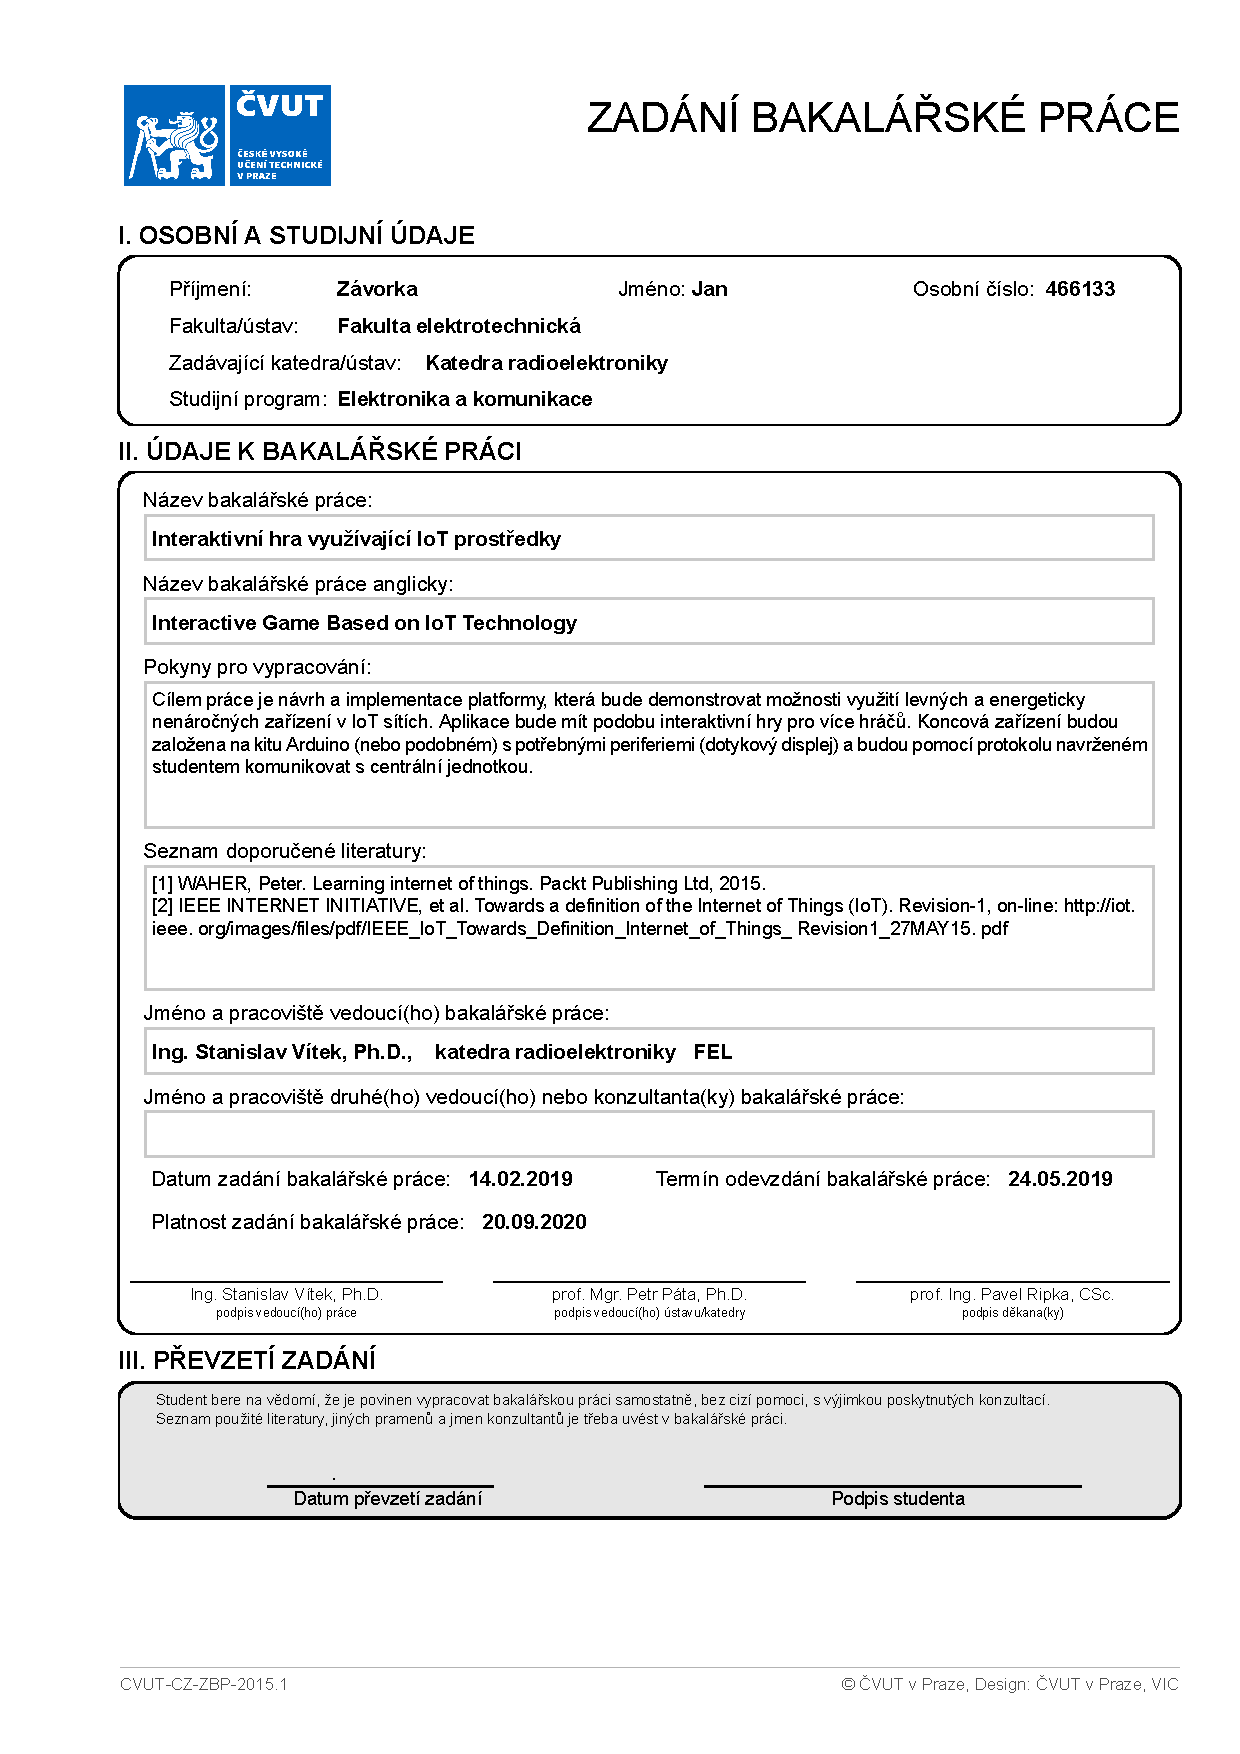
\includepdf{img/zadani_prace.pdf}
\blankpage
\cleardoublepage

\setcounter{page}{0} %cislo strany
\pagestyle{empty} %Nezobrazovat číslo stránky
\newpage ~\vfill „Prohlašuji, že jsem předloženou práci vypracoval samostatně a že jsem uvedl
veškeré použité informační zdroje v souladu s Metodickým pokynem o
dodržování etických principů při přípravě vysokoškolských závěrečných prací.“\\[3em] V~Praze dne \today \hspace{.2\textwidth} \dotfill\\
\hspace*{11cm} Podpis

\newpage

\vspace*{\fill}
\section*{Poděkování}
Děkuji Ing. Stanislavu Vítkovi, Ph.D. za pomoc při vedení bakalářské práce. \\
\noindent
Mé poděkování patří též Ing. Petru Skalovi za cenné rady a pomoc s 3D tiskem.

\newpage

\newpage
\section*{Abstrakt}
Tato bakalářská práce se zabývá vývojem a výrobou jednoduchého zařízení, které umožňuje demostrovat využití energeticky nenáročných zařízení v IoT sítích. Zařízení má podobu jednoduché hry pro více hráčů - piškvorek a je postaveno na platdormě Arduino. Zařízení je realizováno pomocí tří koncových zařízení (klientů) s dotykovými displeji pro interakci s uživatelem a jednoho centrálního řídicího prvku (serveru). V práci je popsán konkrétní použitý hardware včetně návrhu krabiček. Dále je zde podrobně rozepsán vytvořený software včetně možnosti úprav pro použití s jinými moduly. Nakonec je uveden i návod na oživení a obsluhu.\\

\vspace{.5cm}
\noindent
Klíčová slova: Arduino Ethernet, IoT demonstrátor, Arduino hra, Arduino IoT



\section*{Abstract}
{
\selectlanguage{english}
This bachelor thesis deals with development and production simple device which can demostrate usage  of low power devices in IoT networks. This device has form of multiplayer game - Noughts and crosses and is based on Arduino platform. The device has three end nodes (clients) with touch screen for interaction with user and one control device (server). There is descriped used hardware including design of cases for all devices in this thesis. There is also description of software including list of possible changes which could be made for purpose to use this product with different modules. In the end there is manual for starting and operating this device.

\vspace{.5cm}
\noindent
Key words: Arduino Ethernet, IoT demonstration device, Game based on Arduino, Arduino IoT
}

\clearpage

\pagestyle{fancy}

%%%%%%%%%%%%%%%%%%%%%%%%%%%%%%%%%

%%% List of figures, tables, abbriviations %%%%
\pagenumbering{roman}
\tableofcontents
\blankpage
\cleardoublepage

 \listoffigures
 %\blankpage
 %\cleardoublepage

\clearpage
 \listoftables
 %\blankpage
 %\cleardoublepage

% \printglossary[type=\acronymtype,title=Abbreviations,nonumberlist]
% \blankpage
% \cleardoublepage
%%%%%%%%%%%%%


\pagenumbering{arabic}

%\setcounter{figure}{0}
%\setcounter{table}{0}
%\setcounter{equation}{0}
\clearpage
\section{Úvod}
Cílem práce bylo vytvořit zařízení, které by demonstrovalo využití jednodeskových počítačů v IoT sítích. Pro realizaci byla zvolena platforma Arduino. Důvodem pro zvolení této platformy bylo především její rozšíření mezi uživateli a dostupnost doplňkových periferií. Samotné zařízení by mělo mít funkci hry pro více hráčů. Koncová zařízení budou vybavena budou vybavena dotykovým displejem pro interakci s uživatelem. Celá hra pak bude řízena jednou centrální jednotkou taktéž založenou na platformě Arduino. Komunikace mezi jednotlivými zařízeními pak bude probíhat po Ethernetové síti. Pro dobrou názornost a nenáročnost (co se týče složitosti implementace, tak i potřebného hardwarového výkonu) byla zvolena hra piškvorky.

Práce je rozdělena do tří částí. V první části je popsán použitý hardware, včetně jeho případných úprav. Nechybí zde ani popis dalších komponent, které jsou potřeba pro kompletaci celého zařízení. Druhá část je zaměřena na popis softwaru, především na metody komunikace koncových zařízení. Pro názornost jsou některé důležité úkony doplněny diagramy. Poslední část je věnována už samotnému funkčnímu zařízení. Lze zde nalézt návod na zprovoznění, včetně fotografií funkčního prototypu.

%{\color{ashgrey} Nějaké obecné věci o IoT}

Samotný pojem IoT (\uv{Internet of things} - Internet věcí) označuje propojení fyzických zařízení prostřednictvím internetu. Jako koncová fyzická zařízení jsou většinou používány různé vestavěné systémy vybavedené samotným řídicím mikrokontrolérem a řadou senzorů. Tato zařízení dokáží komunikovat jak mezi sebou, tak se zeřízením uživatele (mobilním telefon) nebo dokáží předávat naměřená data na cloud.

IoT samozřejmě není jen o koncových zařízeních, dalším důležitým prvkem jsou brány (\textit{gateway}), které zajišťují spojení mezi koncovými zařízeními a například cloudem. IoT síť lze rozdělit do několika kategorií \cite{iot_geographic} podle fyzického rozmístění:
\begin{itemize}
  \item \textit{nanonetwork} \ldots spojení několika malých (řádově mikrometrů) zařízení, které mají za úkol plnit jednoduché úkony.
  \item \textit{NFC (Near-Field Communication)} \ldots spojení zařízení na vzdálennost řádově jednotky centimetrů.
  \item \textit{BAN (Body Area Network)} \ldots spojení zařízení v oblasti lidského těla, zejména různá nositelná zařízení případně senzory uvnitř těla.
  \item \textit{PAN (Personal Area Network)} \ldots síť v oblasti jedné místnosti.
  \item \textit{LAN (Local Area Network)} \ldots síť v oblasti jedné budovy.
  \item \textit{CAN (Corporate Area Network)} \ldots síť v oblasti jedno kampusu/společnosti, spojuje několik lokální sítí.
  \item \textit{MAN (Metropolitan Area Network)} \ldots síť v oblasti jedno města.
  \item \textit{WAN (Wide Area Network)} \ldots síť pokryvající větší geografickou oblast, spojuje menší sítě.
\end{itemize}
Z tohoto pohledu spadá vytvořená platforma do sítí typu \textit{LAN}. Teoreticky by bylo možné ho připojit například do internetu, problém však je, že zařízení na to není stavěné - nemá implementovány žádné ochranné/šifrovací mechanismy ani žádné autentizační procesy. Díky hardwarové implementaci TCP/IP v kontrolérech WIZnet~\cite{datasheet_w5100} by nemělo docházet k výraznému ovlivnění útoky typu DDoS \cite{ArdIotDDOS}.

Další důležitou součástí IoT je i implementace nových protokolů a standardů pro komunikaci. Mezi nejznámnější lze například zařadit úspornou verzi Bluetooth - \textit{BLE: Bluetooth low energy}, které se používá například u nositelných zařízeních. Dalším, spíše na průmysl zaměřeným, protokolem je \textit{ZigBee}, který je známý díky svému dobrému zabezpečení. Pro použití v rozlehlých sítích s velkým počtem zařízení je vhodný LoRaWAN \cite{IoTprotocols}. I když je na výběr v velké palety  protokolů (lišící se například přenosovými rychlostmi, dosahem), byl pro komunikaci mezi zařízeními vybrán Ethernet.

\cleardoublepage

% \input{state-of-art}
% \cleardoublepage

%\setcounter{figure}{0}
%\setcounter{table}{0}
%\setcounter{equation}{0}
\section{Hardware}
Celá platforma se skládá z jednoho řídicího prvku (viz. kapitola \ref{sec:HWserver}) a třech (maximální počet klientů je hardwarově limitován na čtyři) klientských zařízení (viz. kapitola \ref{sec:HWclient}). Datové spojení je realizováno hvězdicovou topologií (schéma na obrázku \ref{fig:schema_net}). Jako centrální prvek byl použit switch D-Link DGS-105.
Celá demonstrační sestava se pak skládá z:
\begin{itemize}
  \item 1x switch D-Link DGS-105
  \item 1x server s Arduino DUE
  \item 3x klient s Arduino Ethernet a dotykovým displejem
  \item 4x propojuvací UTP kabel
  \item 1x napájecí adaptér pro switch (5 V/1 A součástí balení)
  \item 4x napájecí adaptér 12 V/1500 mA
\end{itemize}

\begin{figure}[hbtp]
  \centering
  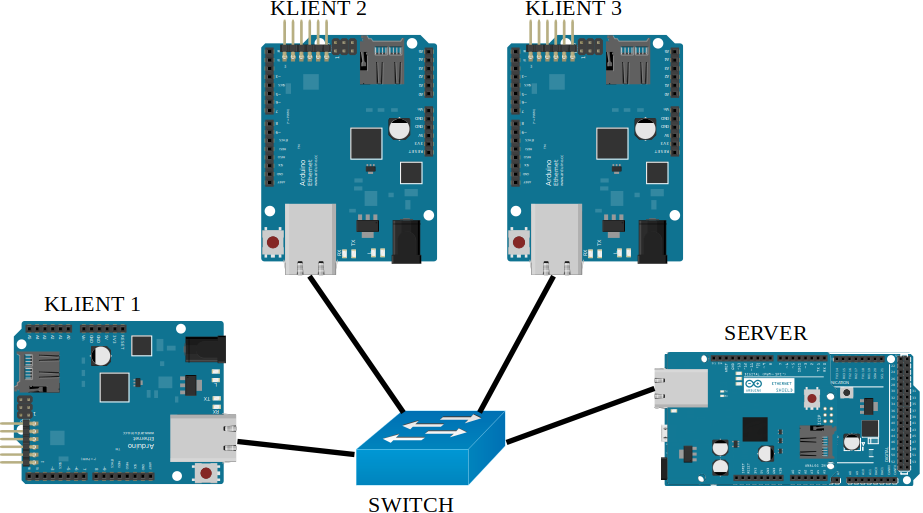
\includegraphics[width=12cm]{img/schema_net.png}
  \caption{\label{fig:schema_net} Schéma zapojení jednotlivých zařízení do sítě, zdroj \cite{fig_ArdEthernet, fig_ArdEthShield, fig_switchIco, fig_ArdDue}}
\end{figure}

\subsection{Zařízení typu server}
\label{sec:HWserver}
Zařízení je založeno na desce \textit{Arduino Due}, které obsahuje mikrokontrolér Atmel SAM3X8E ARM Cortex-M3 s 512 kB flash paměti a nabízí dostatečný výkon pro správné fungování serveru. Původní varianta totiž počítala s nasazením desky \textit{Arduino Ethernet} i jako serveru. To se ovšem vzhledem k omezeným prostředkům ukázalo jako problematické, proto byla zvolena právě deska \textit{Arduino Due}.

Pro připojení do sítě je použit Ethernetový shield s čipem Wiznet W5100, který je přímo napojen na Arduino. Tímto je dána ona limitace maximálně na 4 hráče, protože dle datasheetu výrobce čipu~\cite{datasheet_w5100} je maximální počet spojení právě čtyři. Ethernetový shield komunikuje s Arduinem pomocí SPI sběrnice

Pro pohodlné ovládání jsou k serveru připojena dvě tlačítka a jedna barevná svítivá dioda. Význam jednotlivých stavů svítivé diody a funkce tlačítek je popsána v kapitole~\ref{sec:ovladani}. Propojení těchto periferií s Arduinem je realizováno pomocí jednostrané DPS, schéma zapojení je pak na obrázku~\ref{fig:server_module}.

\begin{figure}[hbtp]
  \centering
  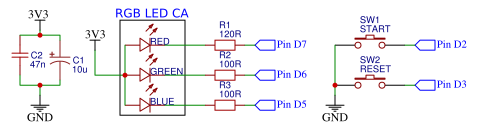
\includegraphics[width=12cm]{img/server_module.png}
  \caption{\label{fig:server_module} Schéma zapojení periferií u serveru}
\end{figure}

Napájení je řešeno externím adaptérem, dle stránek výrobce~\cite{ArdDue_web} je možné pužít napětí 6 - 16 V (využívá se interní stabilizátor), přižemž odběr je kolem 140 mA při napájení 12 V. V případě, že je pro ovládání použita sériová linka (server je připojen USB kabelem k počítači, ovládání tímto způsobem je popsáno v kapitole~\ref{sec:ovladani}), postačuje napájení dodané přes USB kabel a není potřeba připojovat externí napájecí zdroj.

Celé zařízení je pak umístěno v krabičce jejíž návrh je na obrázku~\ref{fig:server_navrh} a realizace na obrázku~\ref{fig:server_realizace}. Krabička byla navrhnuta v programu Autodesk Inventor Professional 2019 Student Edition a realizovaná 3D tiskem na tiskárně Original Prusa i3 MK3S. Krabička je osazena červeným a zeleným tlačítkem, barevnou sívitvou 5~mm diodou (se společnou anodou) a souosým napájecím konektorem 5,5x2,1~mm. Pro upevnění Arduina jsou použity šrouby M2,5x10 a závitové vložky M2,5x6 vtavené do připravených otvorů v krabičce. Arduino deska sice nabízí montážní otvory o průměru 3~mm, ale vzhledem k rozložení součástek zde není dostatek místa pro hlavu šroubu~M3.

%\begin{figure}[hbtp]
%\centering
%\begin{minipage}[c]{\textwidth/2-1cm}
%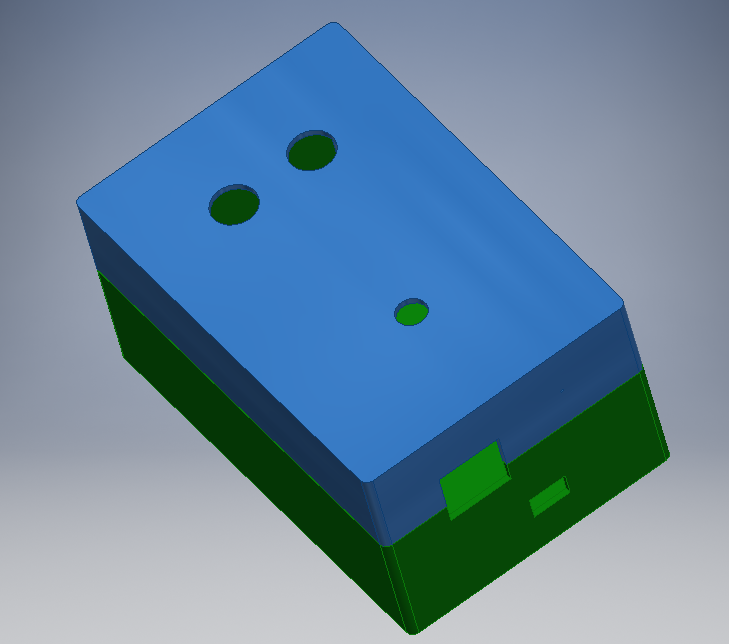
\includegraphics[width=\textwidth]{img/foto/server_navrh.png}
%\end{minipage}
%\begin{minipage}[c]{\textwidth/2-1cm}
%
\includegraphics[width=\textwidth]{img/foto/server_realizace.png}
%\end{minipage}
%\\
%\begin{minipage}[c]{\textwidth/2-0.5cm}
%\caption{\label{fig:server_navrh}Návrh krabičky pro server}
%\end{minipage}
%\begin{minipage}[c]{\textwidth/2-.5cm}
%\caption{\label{fig:server_realizace}Zkompletovaná krabička pro server}
%\end{minipage}
%end{figure}

\begin{figure}[hbtp]
  \centering
  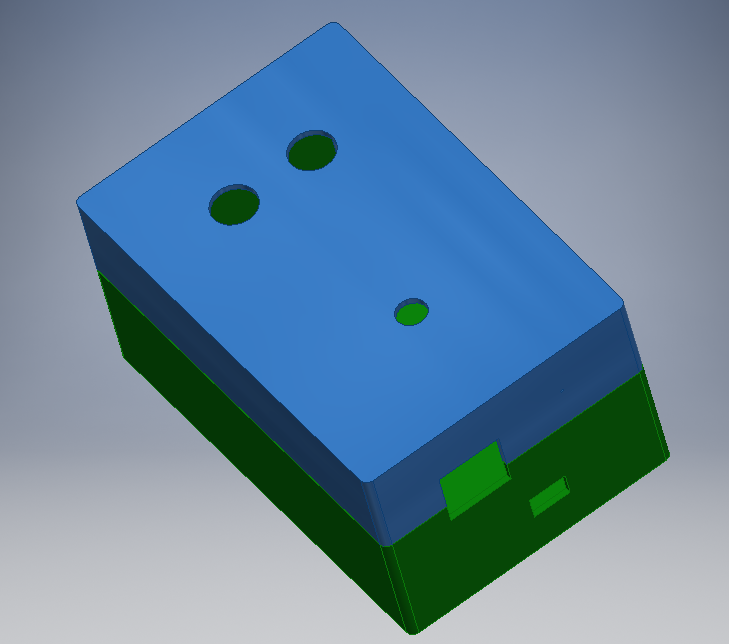
\includegraphics[height=7cm]{img/foto/server_navrh.png}
  \caption{\label{fig:server_navrh}Návrh krabičky pro server}
\end{figure}

\begin{figure}[hbtp]
  \centering
  
\includegraphics[height=7cm]{img/foto/server_realizace.jpg}
  \caption{\label{fig:server_realizace}Zkompletovaná krabička pro server}
\end{figure}


\subsection{Zařízení typu klient}
\label{sec:HWclient}
Zařízení je založeno na desce Arduino Ethernet, která je vybavena mikrokontrolérem ATmega328 s 32 kB flash paměti. Tato deska byla zvolena především kvůli tomu, že má vestavěný ethernetový kontrolér, který tak nezabírá piny pro připojení shieldu s displejem. Malá flash paměť se však během vývoje ukázala jako značně limitující, protože při nahrání všech potřebných knihoven (popsáno v kapitole~\ref{sec:knihovny}) zůstalo k dispozici 30~\% programové paměti. I z tohoto důvodu byla zvolena jako hra piškvorky, která není programově příliš složitá a také bylo nutné vynechat složitější menu například s nastavením barvy nebo změny IP adresy serveru (to se nyní musí provádět změnou v kódu a přeprogramováním Arduina, více v kapitole \ref{sec:client-nastaveni}).

Jak už bylo zméněno výše, tato deska má věstavěný ethernet kontrolér WIZnet, konkrétně typ W5100. U klienta není maximální počet spojení limitující (klient drží pouze jedno spojení se serverem), jedinou nevýhodou kontroléru W5100 tak zůstává, že neobsahuje registr, ve kterém je uložena informace o fyzickém připojení ethernetového kabelu k desce \cite{datasheet_w5100}. Tím je zkomplikována detekce připojení a odpojení kabelu a zůstává tak pouze možnost vizuální kontroly pomocí svítivých diod na konektoru RJ-45.

Pro interakci s uživatelem je klient vybaven 2,4" barevným TFT LCD displej s rozlišením 320x240 pixelů s rezistivní dotykovou plochou. Displej je vybaven  řadičem SUM74HC245T. Vzhledem k rozměrům (výšce) RJ-45 konektoru, který je umístěn na desce, je nutné pro správné připojení použít lištu oboustrannými kolíky o délce kolíku minimálně 15~mm. Protože u displejů použitých v tomto projektu byly kolíky připájeny už od výrobce, byla dodatečně vyrobená patice s dutinkové lišty a lišty s oboustrannými kolíky.

Pro napájení byl zvolen externí napájecí adaptér, avšak připojení na integrovaný stabilizátor není možné, protože Arduino s displejem při 5~V odebírá přibližně 400~mA, což integrovaný stabilizátor nedokáže poskytnout (vlivem velého ztrátového výkonu dochází k jeho značnému zahřívání). Napájení přímo napětím 5~V není také příliš vhodné, protože vlivem například ztrát přívodních vodičů může dojít ke kolísání napětí, tím dojde i k pohybu reference AD převodníku připojenému k dotykové vrstvě displeje a tak může docházet k nesprávnému vyhodnocení stisku (může se lišit reálné místo stisku od toh, které vyhodnotil mikrokontrolér). Jako nejlepší varianta se ukázalo použití modulu se snižujícím DC-DC měničem. Modul obsahuje spínací regulátor MP1584 a dle dodavatele je schopen pracovat s napětím 6~-~25~V (při výstupním napětí 5~V) a dodat proud až 1,5~A, což je pro tuto aplikaci dostačující.

Stejně jako v případě serveru je celé zařízení umístěno ve vytištěné krabičce, návrh a realizovaná krabička jsou na obrázcích \ref{fig:client_navrh}, \ref{fig:client_realizace}. Princpi uchycení Arduina je stejný jako v případě serveru, pro napájení je opět osazen souosý napájecí konektor 5,5x2,1~mm. Dále je z boku výřez por konektor RJ-45 pro připojení do ethernetové sítě a na vrchu se nachází výřez pro displej vedle kterého se je umístěn otvor pro přístup k resetovacímu tlačítku.

%\begin{figure}[hbtp]
%\centering
%\begin{minipage}[c]{\textwidth/2-1cm}
%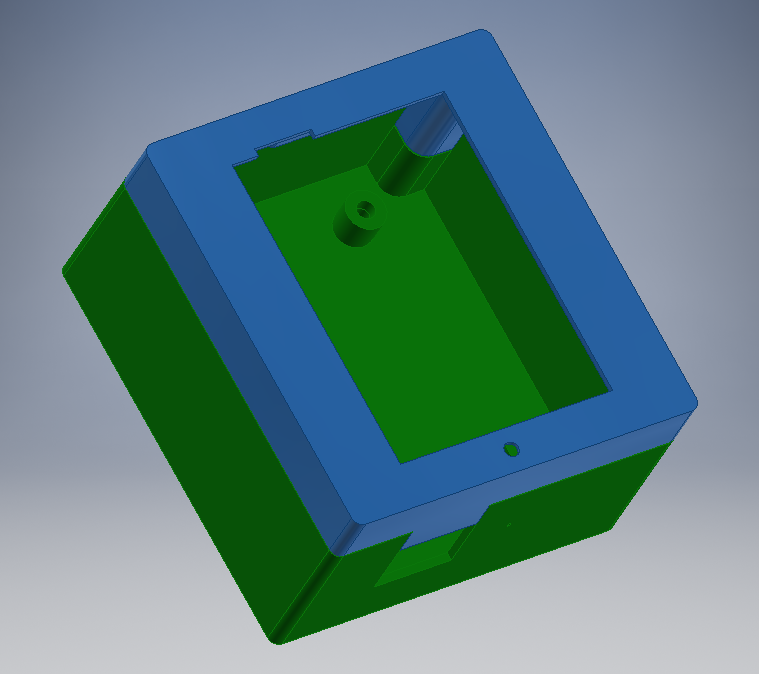
\includegraphics[width=\textwidth]{img/foto/client_navrh.png}
%\end{minipage}
%\begin{minipage}[c]{\textwidth/2-1cm}
%
\includegraphics[width=\textwidth]{img/foto/client_realizace.png}
%\end{minipage}
%\\
%\begin{minipage}[c]{\textwidth/2-0.5cm}
%\caption{\label{fig:client_navrh}Návrh krabičky pro klienta}
%\end{minipage}
%\begin{minipage}[c]{\textwidth/2-.5cm}
%\caption{\label{fig:client_realizace}Zkompletovaná krabička pro klienta}
%\end{minipage}
%\end{figure}

\begin{figure}[hbtp]
  \centering
  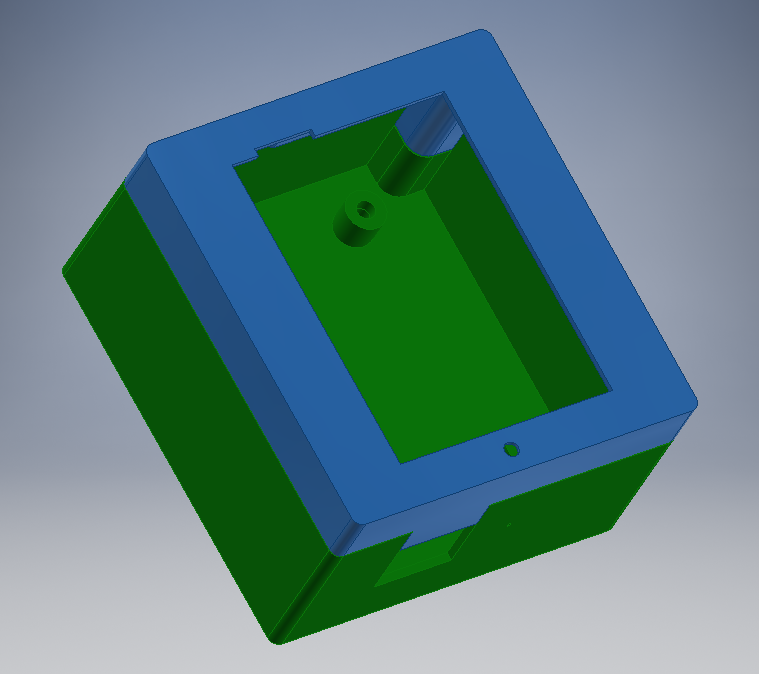
\includegraphics[height=7cm]{img/foto/client_navrh.png}
  \caption{\label{fig:client_navrh}Návrh krabičky pro klienta}
\end{figure}

\begin{figure}[hbtp]
  \centering
  
\includegraphics[height=7cm]{img/foto/client_realizace.jpg}
  \caption{\label{fig:client_realizace}Zkompletovaná krabička pro klienta}
\end{figure}

\cleardoublepage

%\setcounter{figure}{0}
%\setcounter{table}{0}
%\setcounter{equation}{0}
\section{Popis softwaru}
\subsection{Knihovny}
Pro realizaci byly použity následující knihovny:
\begin{itemize}
  \item \textit{Ethernet library}: knihovna slouží pro připojení Arduina k internetu. Jak je uvedeno na webových stránkách \cite{EthLib} jsou podporovány desky a shieldy založené na konrolérech W5100, W5200, W5500. Tato knihvna je použita jak u serveru tak i u klientů. U serveru připojený ethernet shield obsadí piny 10, 11, 12, 13. Komunikace Arduina se shieldem (ethernet kontrolérem) probíhá po SPI sběrnici.

  \item \textit{MCUFRIEND\_kbv library}: knihovna slouží k ovládání displeje u klienta. Pro správnou funkci je nutné, jak se zmiňuje autor na domovské stránce knihovny~\cite{lib_MCUFRIEND_kbv}, je nutné mít k dispozici také knihovnu \textit{Adafruit\_GFX} \cite{lib_adafruitGFX}. Pro použití displeje se nejdříve vytvoří instance třídy \texttt{UTFGLUE}, kde je nutné správně definovat piny pro daný shield, v tomto případě \texttt{UTFTGLUE LCD(0x0154,A2,A1,A3,A4,A0);}. Pro řízení displeje jsou pak volány patřičné metody formou \textit{LCD.metoda(parametry);}, například pro vyplnění celého displeje černou \texttt{LCD.clrScr();}. Pomocí ukázkouvého zdrojového kódu z této knihovny \textit{(examples/TouchScreen\_
calibr\_kbv)} byly získány kalibrační hodnoty pro dotykovou plochu displeje.

  \item \textit{Adafruit\_TouchScreen}: slouží k zaznamenání hodnot ze čtyřvodičové dotykové plochy. Stejně jako u knihovny pro displej je nejdříve nutné vytvořit instanci dané třídy \texttt{TouchScreen} v tomto případě tak \texttt{TouchScreen Touch(XP, YP, XM, YM, 300);}, kde \textit{XP, YP, XM, YM} jsou piny, na které je vyvedená dotyková plocha (pro použitý shield jsou to: XP = 6, YP = A1, XM = A2, YM = 7). Hodnota 300 by pak dle popisu knihovny \cite{lib_touch} označuje elektrický odpor dotykové plochy X (měřeno multimetrem mezi piny XP a XM). Pro použité shiledy je hodnota přibližně $300  \ \mathrm{\Omega}$. Dále je třeba určit minimální a maximální tlak pro vyhodnocení dotyku pomocí \texttt{\#define MINPRESSURE} a \texttt{\#define MAXPRESSURE}. Vyhovující jsou hodnoty uvedené v ukázkových kódech pro knihovnu a to konkrétně 10 pro \texttt{MINPRESSURE} a 1000 pro \texttt{MAXPRESSURE}.

  \item \textit{SimpleTimer Library for Arduino}: jednoduchá knihovna, která slouží k řízení určitých časových událostí (kde není třeba velká přesnot), například pro zobrazení a skrytí chybových hlášek, blikání indikační svítivé diody u serveru. Dle webových stránek \cite{lib_simpleTimer} je knihovna založená na funkci \texttt{milis();} (vrací počet milisekund od začátku běhu programu) a nevyužívá přerušení ani harwarový timer.
\end{itemize}

\subsection{Konfigurační hodnoty}
V této kapitole jsou popsány jednotlivé konfigurační hodnoty, která by mohlo být třeba upravit pro správnou funkci celého zařízení. Změny se vždy provádí přímo ve zdrojovému kódu, vždy pouze v hlavní souboru: \textit{piskvorky\_MP\_client.ino} pro klienta a \textit{piskvorky\_MP\_server.ino} pro server. Jak už bylo zmíněno v kapitole \ref{sec:HWclient}, nebylo možné, kvůli malé paměti pro program, implementovat menu, proto je nutné změny provádět přímo ve zdrojovém kódu a dané zařízení pak přeprogramovat. V případě serveru je k dispozici microUSB konektor, který je dostupný skrze obdélníkový otvor na boku zařízení. V případě clienta je nutné demontovat víko, odpojit napájecí modul (v modré bužírce) a připojit Arduino k počítači pomocí převodníku USB - UART.

Jednotlivé konfigurační bloky jsou vždy ohraničeny komentáři mezi nimiž se nacházejí jednotlivé proměnné a popis jejich funkce a omezení hodnot. Níže je uveden příklad ohraničení bloku pro nastavení sítě (IP adresa a port):
\begin{verbatim}
/* ---------- KONFIGURACE - nastavení sítě ----------*/

/* ---------- KONEC - nastavení sítě ----------*/
\end{verbatim}


\subsubsection{Konfigurace serveru}
\label{sec:server-nastaveni}
%Nastavení sítě
V prvním případě je nutné vybrav síťový režim, v případě \textit{ETHMODE\_STATIC} je použita IP adresa, která je uložena v proměnné \textit{serverAddress}. V případě volby \textit{ETHMODE\_DHCP} je adresa přiřazena DHCP serverem a je nutné dodržet aby se přiřazená adresa neměnila a byla zároveň nastavená u jednotlivých klientů.

Dále je třeba nastavit příslušnou MAC adresu, v případě použitého nebyla přiřazena výrobcem, takže je nutné nějakou zvolit. Vzhledem k tomu, že zařízení se provozuje na samostatné lokální síti, byla MAC adresa vybrána náhodně, v případě, že v síti jsou další zařízení, je možné vybrat MAC adresu například podle postupu popsaného v \cite{vyberMAC}. Vezme se MAC adresa nějaké zařízení v síti a poslední bajt se zvětší o jedna a takto vzniklá MAC adresa se přiřadí shieldu.
Vybraná MAC adresa je v poli \texttt{mac}.

Jako poslední je potřeba přiřadit port, na kterém budou zařízení komunikovat. Dle normy \cite{norm_RFC6335} je možné zvolit jakoukýkoliv dynamický port (49152-65535), protože tyto porty nebudou nikdy přiřazeny žádné službě. Port je uložen v proměnné \texttt{localPort} a stejný port musí být nastaven i u clientů.
\lstinputlisting[language=C++, style=customc_config, firstline=1, lastline=8, title= Blok konfigurace ethernet shieldu pro server]{codes/server_config.cpp}

%Nastavení pinů
Jak je popsáno v kapitole \ref{sec:HWserver}, jsou k serveru připojena dvě tlačítka a jedna barevná svítivá dioda. V případě, že je nutné tyto periferie připojit jinak, je možné změnit čísla pinů v kofiguračním bloku \textit{nastavení pinů a LED}. Tlačítka využívají interní pull-up rezistory a jejich zapojení je uvedeno na obrázku \ref{fig:server_module}.
\lstinputlisting[language=C++, style=customc_config, firstline=10, lastline=22, title= Blok konfigurace pinů pro svítivou diodu a tlačítka]{codes/server_config.cpp}

%Nastavení barev
Jako poslední je možné nastavit jakou barvu budou mít jednotliví klienti. V ukázkové případě jsou barvy přiřazeny z výběru, který je uveden v kódu, ale je možné také definovat vlastní ve formátu RGB565 (16-bit barva).
\lstinputlisting[language=C++, style=customc_config, firstline=24, lastline=30, title= Blok konfigurace jednotlivých barev pro klienty/hráče]{codes/server_config.cpp}

\subsubsection{Konfigurace klienta}
\label{sec:client-nastaveni}
%Nastavení profilů
Klientů se v celé sestavě nachází několik (v tomto případě tři) a liší se pouze určitým nastavením (IP adresa, MAC adresa, kalibrační hodnoty displeje) proto jsou vytvořeny profily pro jednotlivé klienty (softwarově omezeno na pět). Každému profilu se nastaví požadované parametry a při nahrávání programu do Arduina se pak profily mění pomocí \texttt{\#define CLIENTx}, kde x je číslo jednotlivých klientů/profilů. Pokud není zvolen žádný profil, použití je defaultní hodnoty a uživatel je o tom informován při překladu pomocí direktivy \texttt{\#warning} (zobrazí se hlášení, ale překlad neukončí).
\lstinputlisting[language=C++, style=customc_config, firstline=1, lastline=3, title= Blok výběru profilu pro klienta]{codes/client_config.cpp}

%Nastavení MAC adres
V této části se přiřazují jednotlivé MAC adresy daným profilům. Výhodou oficiálních Arduino Ethernet desek je, že mají MAC adresu přidělenou výrobcem a je možné jí nalézt na bílém štítku ze spodní strany.
\lstinputlisting[language=C++, style=customc_config, firstline=6, lastline=38, title= Blok přiřazení MAC adres jednotlivým klientským profilům]{codes/client_config.cpp}

%Nastavení IP adres
Stejně jako v případě serveru i zde je možné vybrat ze dvou režimů sítě a to \textit{ETHMODE\_STATIC} a \textit{ETHMODE\_DHCP}. V případě volby \textit{ETHMODE\_DHCP} není na adresu přiřazenou DHCP serverem kladen žádný zvláštní nárok. V případě použití \textit{ETHMODE\_STATIC} je ještě nutné dodefinovat IP adresy pro jednotlivé klienty. Opět lze s výhodou využít profilů, pokud se použije defaultní, je o tom uživatel opět při překladu informován.
Kromě toho je ještě nutné doplnit IP adresu serveru, ke kterému se budou klienti připojovat. Ta byla nastavena při konfiguraci serveru (kapitola \ref{sec:server-nastaveni}) stejně tak jako port, který je také nutné zvolit stejný.
\lstinputlisting[language=C++, style=customc_config, firstline=40, lastline=66, title= Blok nastavení síťového režimu a IP adres]{codes/client_config.cpp}

%Nastavení kalibrace displeju
Jako poslední je nutné nastavi kalibrační hodnoty dotykové plochy displeje. Nejjednodušší způsob jejich získání je použít ukázkový program v knihovně \textit{MCUFRIEND\_kbv library}, který lze nalézt  v \textit{(examples/TouchScreen\_
calibr\_kbv)}. V ukázkovém programu je třeba upravit podle použitého shiledu nastavení pinů. Poté stačí postupovat podle pokynů na displeji a výsledek se vypíše na sériovou linku (lze použítintegrovaný v Arduino IDE - \textit{Tools->Serial Monitor}). Krom kalibračních hodnot je také nutné doplnit orientaci displeje (\texttt{\#define TOUCH\_LANDSCAPE} nebo \texttt{\#define TOUCH\_PORTRAIT}), v případě, že nebude zvolena ani jedna možnou, překlad budou ukončen a vypsána chybová hláška (direktiva \texttt{\#error}). I v tomto případě lze s výhodou využít profilů.
\lstinputlisting[language=C++, style=customc_config, firstline=68, lastline=109, title= Blok nastavení kalibračních hodnot dotykové plochy]{codes/client_config.cpp}

\subsection{Komunikace server - klient}
\label{sec:comm_server-client}
Server komunikuje s klienty pomocí pole \textit{board}. Jedná se o jednorozměrné pole typu \textit{byte} o velikosti 136 (velikost musí být dělitelná osmi). V tomto poli jsou vyplněné všechny důležité informace o stavu hry i jednotlivých hráčích, význam jednotlivých hodnot v poli \textit{board} je popsán v tabulce \ref{tab:packet_server-client}.

Při odesílání je toto pole rozděleno na části po osmi bajtech. Každá tato část je vybavena pořadovým číslem a dvoubajtovým kontrolním součtem (v něm je zahrnuto i pořadové číslo) a následně odeslána připojeným klientům.

Klienti postupně přijímají všechny části a v případě bezchybného příjmu data vyhodnotí. V případě, že klient na základě kontrolního součtu identifikoval chybnou část, odešle podle pravidel komunikace klient->server (popsáno v kapitole \ref{sec:comm_client-server}). Server pak v případě přijetí požadavku odešle danému klientovi vyžadovanou část pole.

\begin{table}[hbtp]
\catcode`\-=12
\caption{\label{tab:packet_server-client}Rozložení pole \textit{board} pro přenos dat a řízení hry mezi serverem a klientem}
\begin{tabular}{|c|c|l|}
\hline
Index   & Hodnoty     & \multicolumn{1}{c|}{Popis}                                      \\ \hline
0-89    &             & Každý index odpovídá jednomu čtverečku na herní desce piškvorek \\ \cline{2-3}
        & 0           & Pole je prázdné (neobsazené)                                    \\ \cline{2-3}
        & 1-5         & Obsazeno některým hráčem/klientem                               \\ \hline
90      &             & Přenos řídicí informace pomocí kódu                             \\ \cline{2-3}
        & 0           & nic nedělat                                                     \\ \cline{2-3}
        & 1           & Vše je OK, překreslit obrazovku                                 \\ \cline{2-3}
        & 3           & Příprava nové hry, zobrazit úvodní obrazovku                    \\ \cline{2-3}
        & 9           & Informace pro hráč odpojen, že bude odpojen                     \\ \cline{2-3}
        & 100         & Hra skončila remízou                                            \\ \cline{2-3}
        & 10x         & Hodnota podle hráče, který vyhrál: 101-105 ('x' je číslo hráče) \\ \cline{2-3}
        & 20x         & Problémy/odpojení s daného hráče: 201-205 ('x' je číslo hráče)  \\ \hline
91      & 1-5         & Číslo hráče, který je na tahu, pokud je 0, nikdo nehraje        \\ \hline
93      & 0-89        & Počet odehraných kol (vyplňuje server)                          \\ \hline
95-96   &             & Barva hráče 1                                                   \\ \cline{1-1} \cline{3-3}
97-98   &             & Barva hráče 2                                                   \\ \cline{1-1} \cline{3-3}
99-100  & Kód barvy   & Barva hráče 3                                                   \\ \cline{1-1} \cline{3-3}
101-102 &             & Barva hráče 4                                                   \\ \cline{1-1} \cline{3-3}
103-104 &             & Barva hráče 5                                                   \\ \hline
105-108 &             & IP adresa hráče 1                                               \\ \cline{1-1} \cline{3-3}
109-112 &             & IP adresa hráče 2                                               \\ \cline{1-1} \cline{3-3}
113-116 & IPv4 adresa & IP adresa hráče 3                                               \\ \cline{1-1} \cline{3-3}
117-120 &             & IP adresa hráče 4                                               \\ \cline{1-1} \cline{3-3}
121-124 &             & IP adresa hráče 5                                               \\ \hline
\end{tabular}
\end{table}


\subsection{Komunikace klient - server}
\label{sec:comm_client-server}
Klient komunikuje se serverem, až na výjimku při sestavení spojení, prostřednictvím dvoubajtového pole. Popis jednotlivých částí pole je v tabulce \ref{tab:clietn-server}. Pro kontrolu přenosu se každá zpráva odešle třikrát. Na straně serveru se pak porovnají dvě ze tří přijatých zpráv a ostatní přijatá data se zahodí. Klient může poslat data maximálně jednou za sekundu (posláním dat se rozumí odeslání tří stejných zpráv).

Pokud při porovnání server zjistí, že přijeté zprávy nejsou stejné, odešle danému klientovi znovu herní desku. V případě, že byl daný hráč na tahu a přenos požadavku na vyplnění pole se nezdařil, je mu prostřednictvím znovuodeslání pole znovu aktivován tah.

V případě, že klient přijal od serveru chybná data, odešle požadavek ve tvaru \mbox{\{20, x\}}, kde \textit{x} je číslo chybně přijaté části pole.

\begin{table}[hbtp]
\catcode`\-=12
\caption{\label{tab:clietn-server} Rozložení packetu pro komunikaci klient - server}
\begin{tabular}{|c|c|l|}
\hline
Index & Hodnoty                         & \multicolumn{1}{c|}{Popis}                                                                                                                                                                                \\ \hline
0     & 10                              & \begin{tabular}[c]{@{}l@{}}Jedná se o informaci, že další přenesený bajt bude číslo vyplněné\\ herní pozice v poli \textit{board}    \end{tabular} \\ \cline{2-3}
      & 20                              & \begin{tabular}[c]{@{}l@{}}Žádost klienta o poslání dané části herního pole (board), v další \\ bajtu je číslo dané části \textit{boardu}   \end{tabular}   \\ \hline
1     & \multicolumn{1}{l|}{0-89, 0-16} & \begin{tabular}[c]{@{}l@{}}Podle hodnoty předchozího bajtu: index vyplněného \\ pole nebo pořadí packetu, který má být poslán znovu\end{tabular}                                                          \\ \hline
\end{tabular}
\end{table}



\subsection{Sestavení spojení}
\inProgress

\subsection{Průběh hry}
\inProgress

\cleardoublepage

%\setcounter{figure}{0}
%\setcounter{table}{0}
%\setcounter{equation}{0}
\section{Oživení a obsluha}
\label{sec:ovladani}
Příprava ke spuštění probíhá v několika krocích:
\begin{enumerate}
  \item Připraví se centrální jednotka (v tomto případě switch) a k ní se pomocí síťového kabelu připojí všechna zařízení (klienti i server). Zapojení znázorněno na obrázku \ref{fig:schema_net}.

  \item Připojit napájení k serveru i klientům, pro server napájení 6~-~16~V~DC schopné dodat alespoň 250~mA, pro klienty 6~-~25~V~DC alespoň 500~mA.

  \item Pokud je vše v pořádku, na serveru svítí svítivá dioda modrou barvou a na displejích klientů je úvodní obrazovka s tlačítkem \uv{\textit{PRIPOJIT}} (viz. obrázek \label{fig:faze1}).
\end{enumerate}

\subsection{Ovládání klienta}
\begin{enumerate}
\item Po úspěšném zapnutí se vykreslí úvodní obazovka. (obrázek:~\ref{fig:faze1}).  Zobrazeny jsou informace o nastavené IP adrese serveru a o IP adrese klienta (podle režimu přiřazena DHCP serverem nebo ručně).
\begin{figure}[H]
\centering
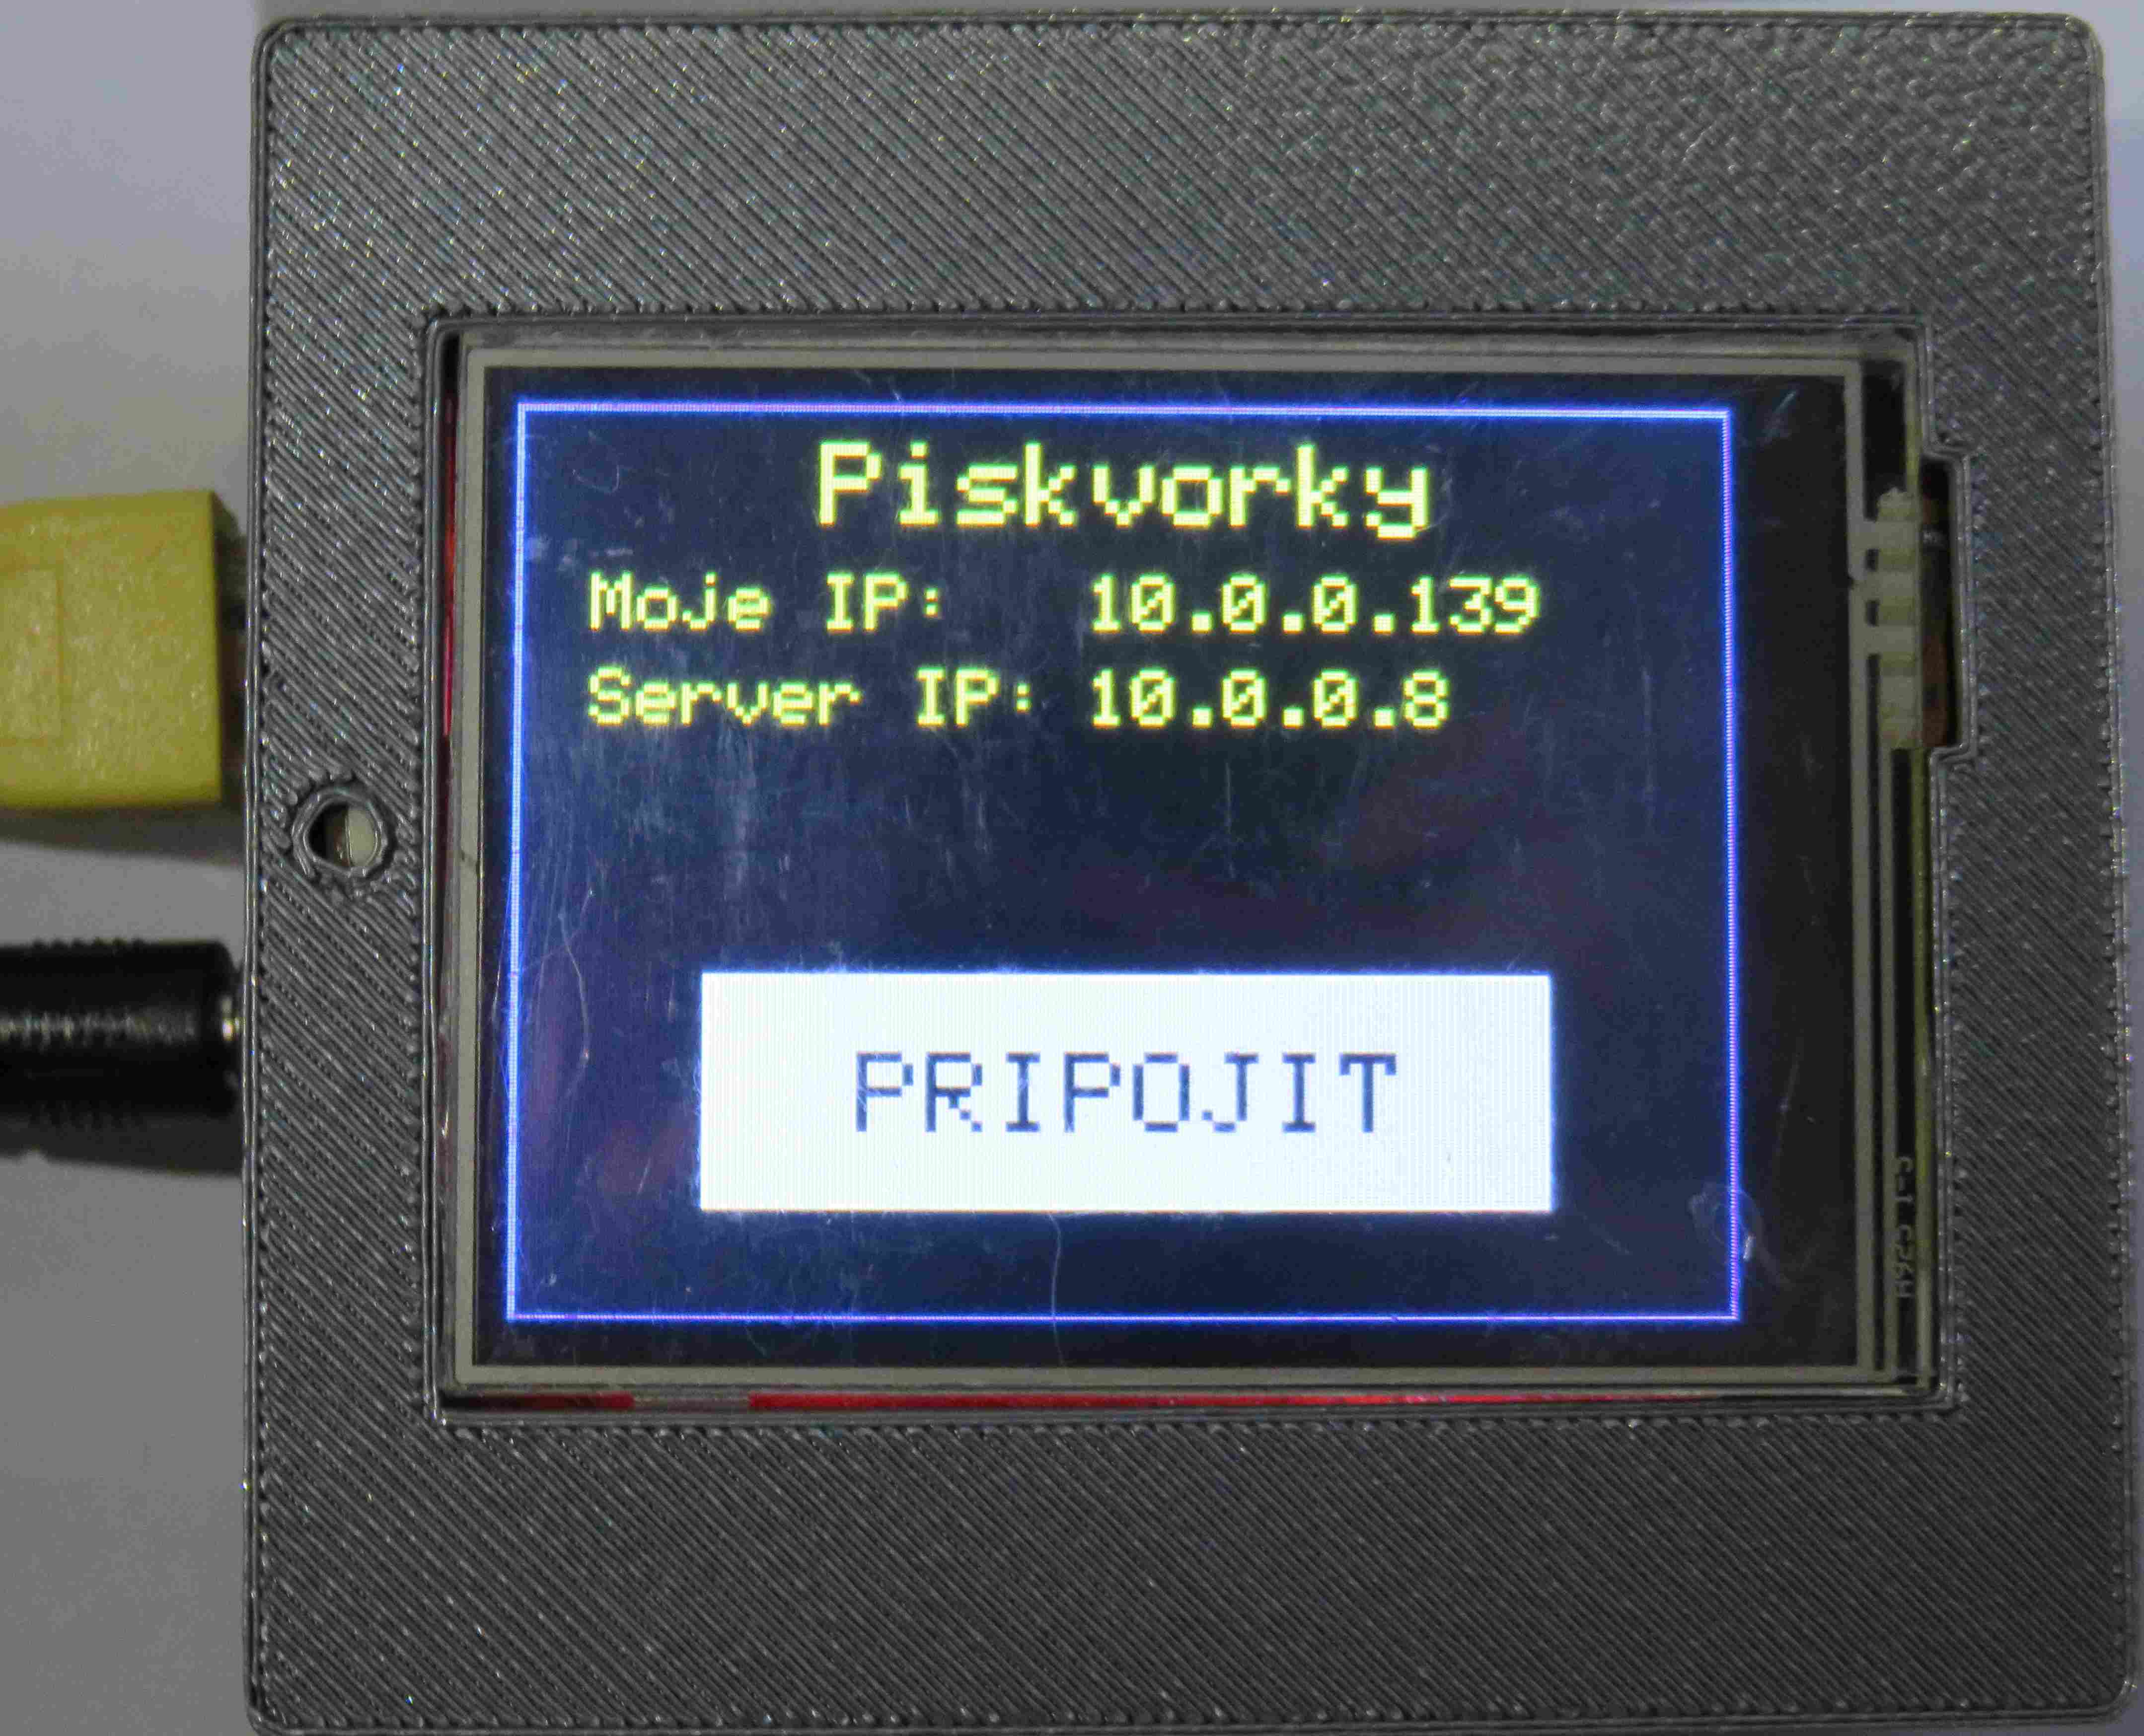
\includegraphics[width=8cm]{img/gameFlow/phase01.jpg}
\caption{\label{fig:faze1} Obrazovka klienta po úspěšném spuštění}
\end{figure}

%%%
\item Připojení k piškvorkovému serveru lze spustit stisknutím tlačítka \uv{\textit{PRIPOJIT}}. Připojování je indikováno pomocí displeje (obrázek~\ref{fig:faze2}). Připojování může být kdykoliv přerušeno stiskem tlačítka \uv{\textit{PRERUSIT}}. Připojování bude dokončeno pokud na serveru není rozehraná hra.
\begin{figure}[H]
\centering
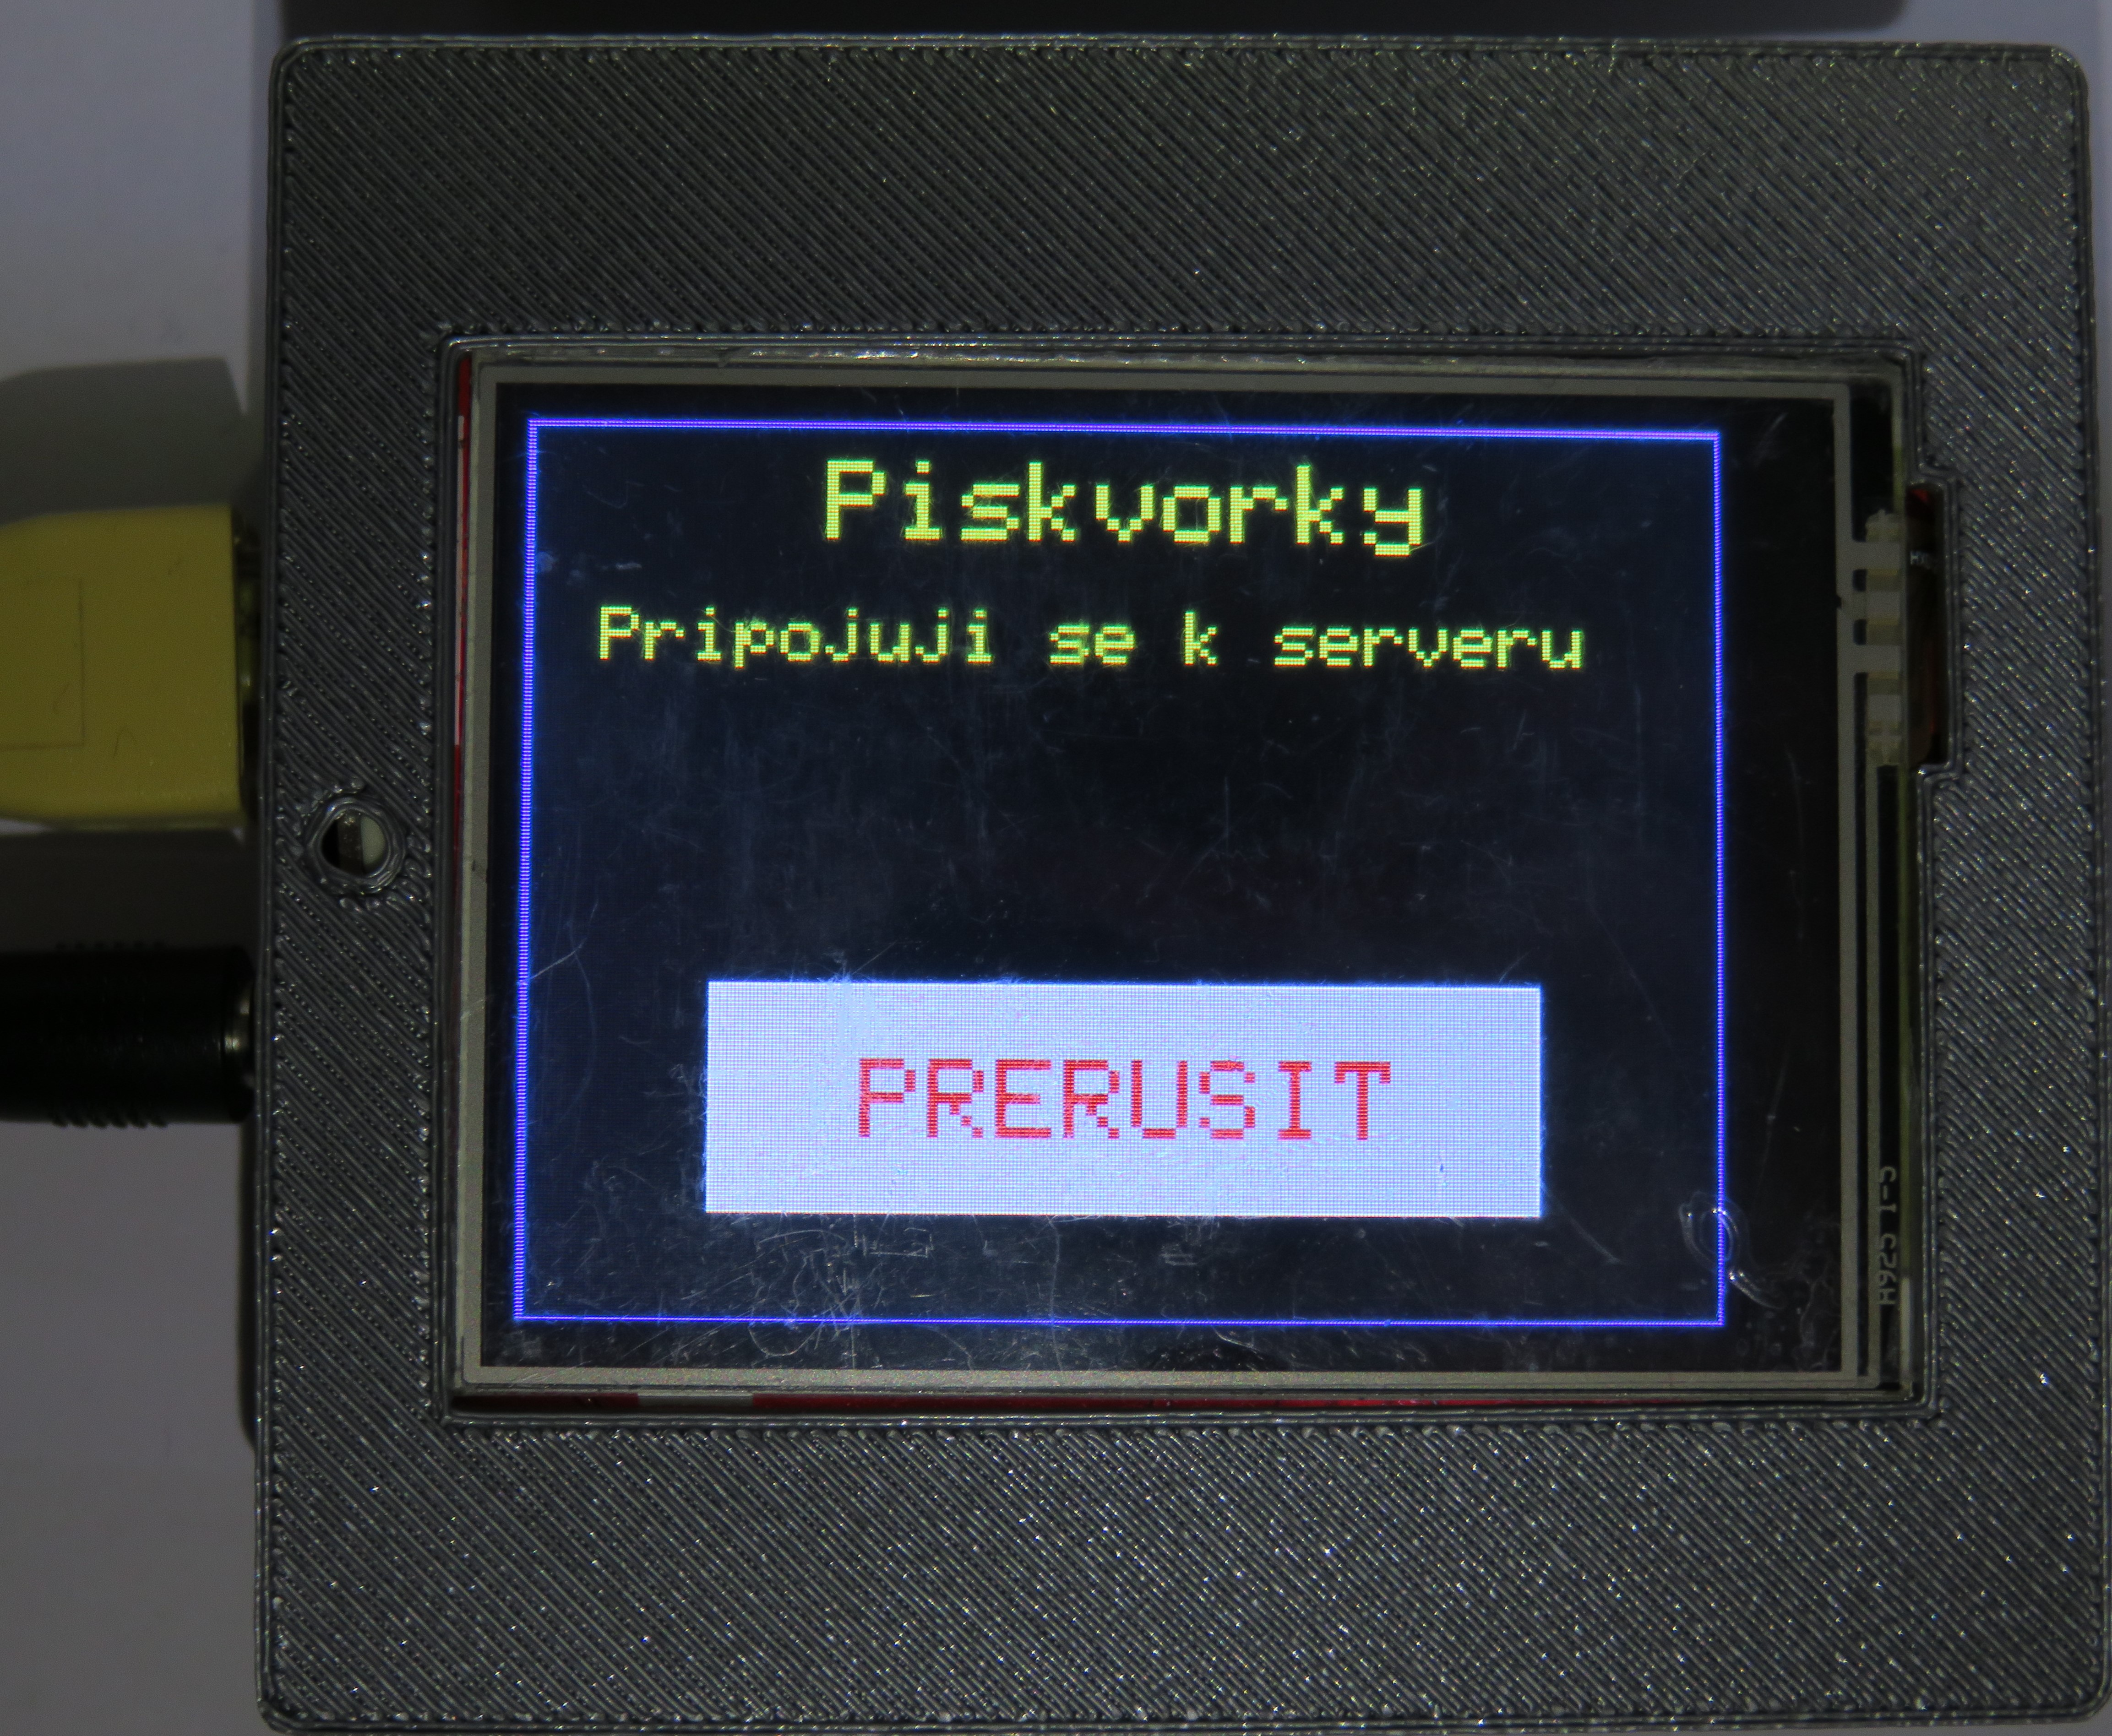
\includegraphics[width=8cm]{img/gameFlow/phase02.jpg}
\caption{\label{fig:faze2} Obrazovka klienta při připojování k serveru}
\end{figure}

%%%
\item Pokud připojení proběhlo úspěšně, klient má od serveru přiřazené číslo a barvu. To je indikováno pomocí displeje (obrázek~\ref{fig:faze3}), kde barva textu odpovídá barvě hráče. Než započne hra je možné se ze serveru odpojit stiskem tlačítka \uv{\textit{ODPOJIT}}. Nyní se čeká na zahájení hry.
\begin{figure}[H]
\centering
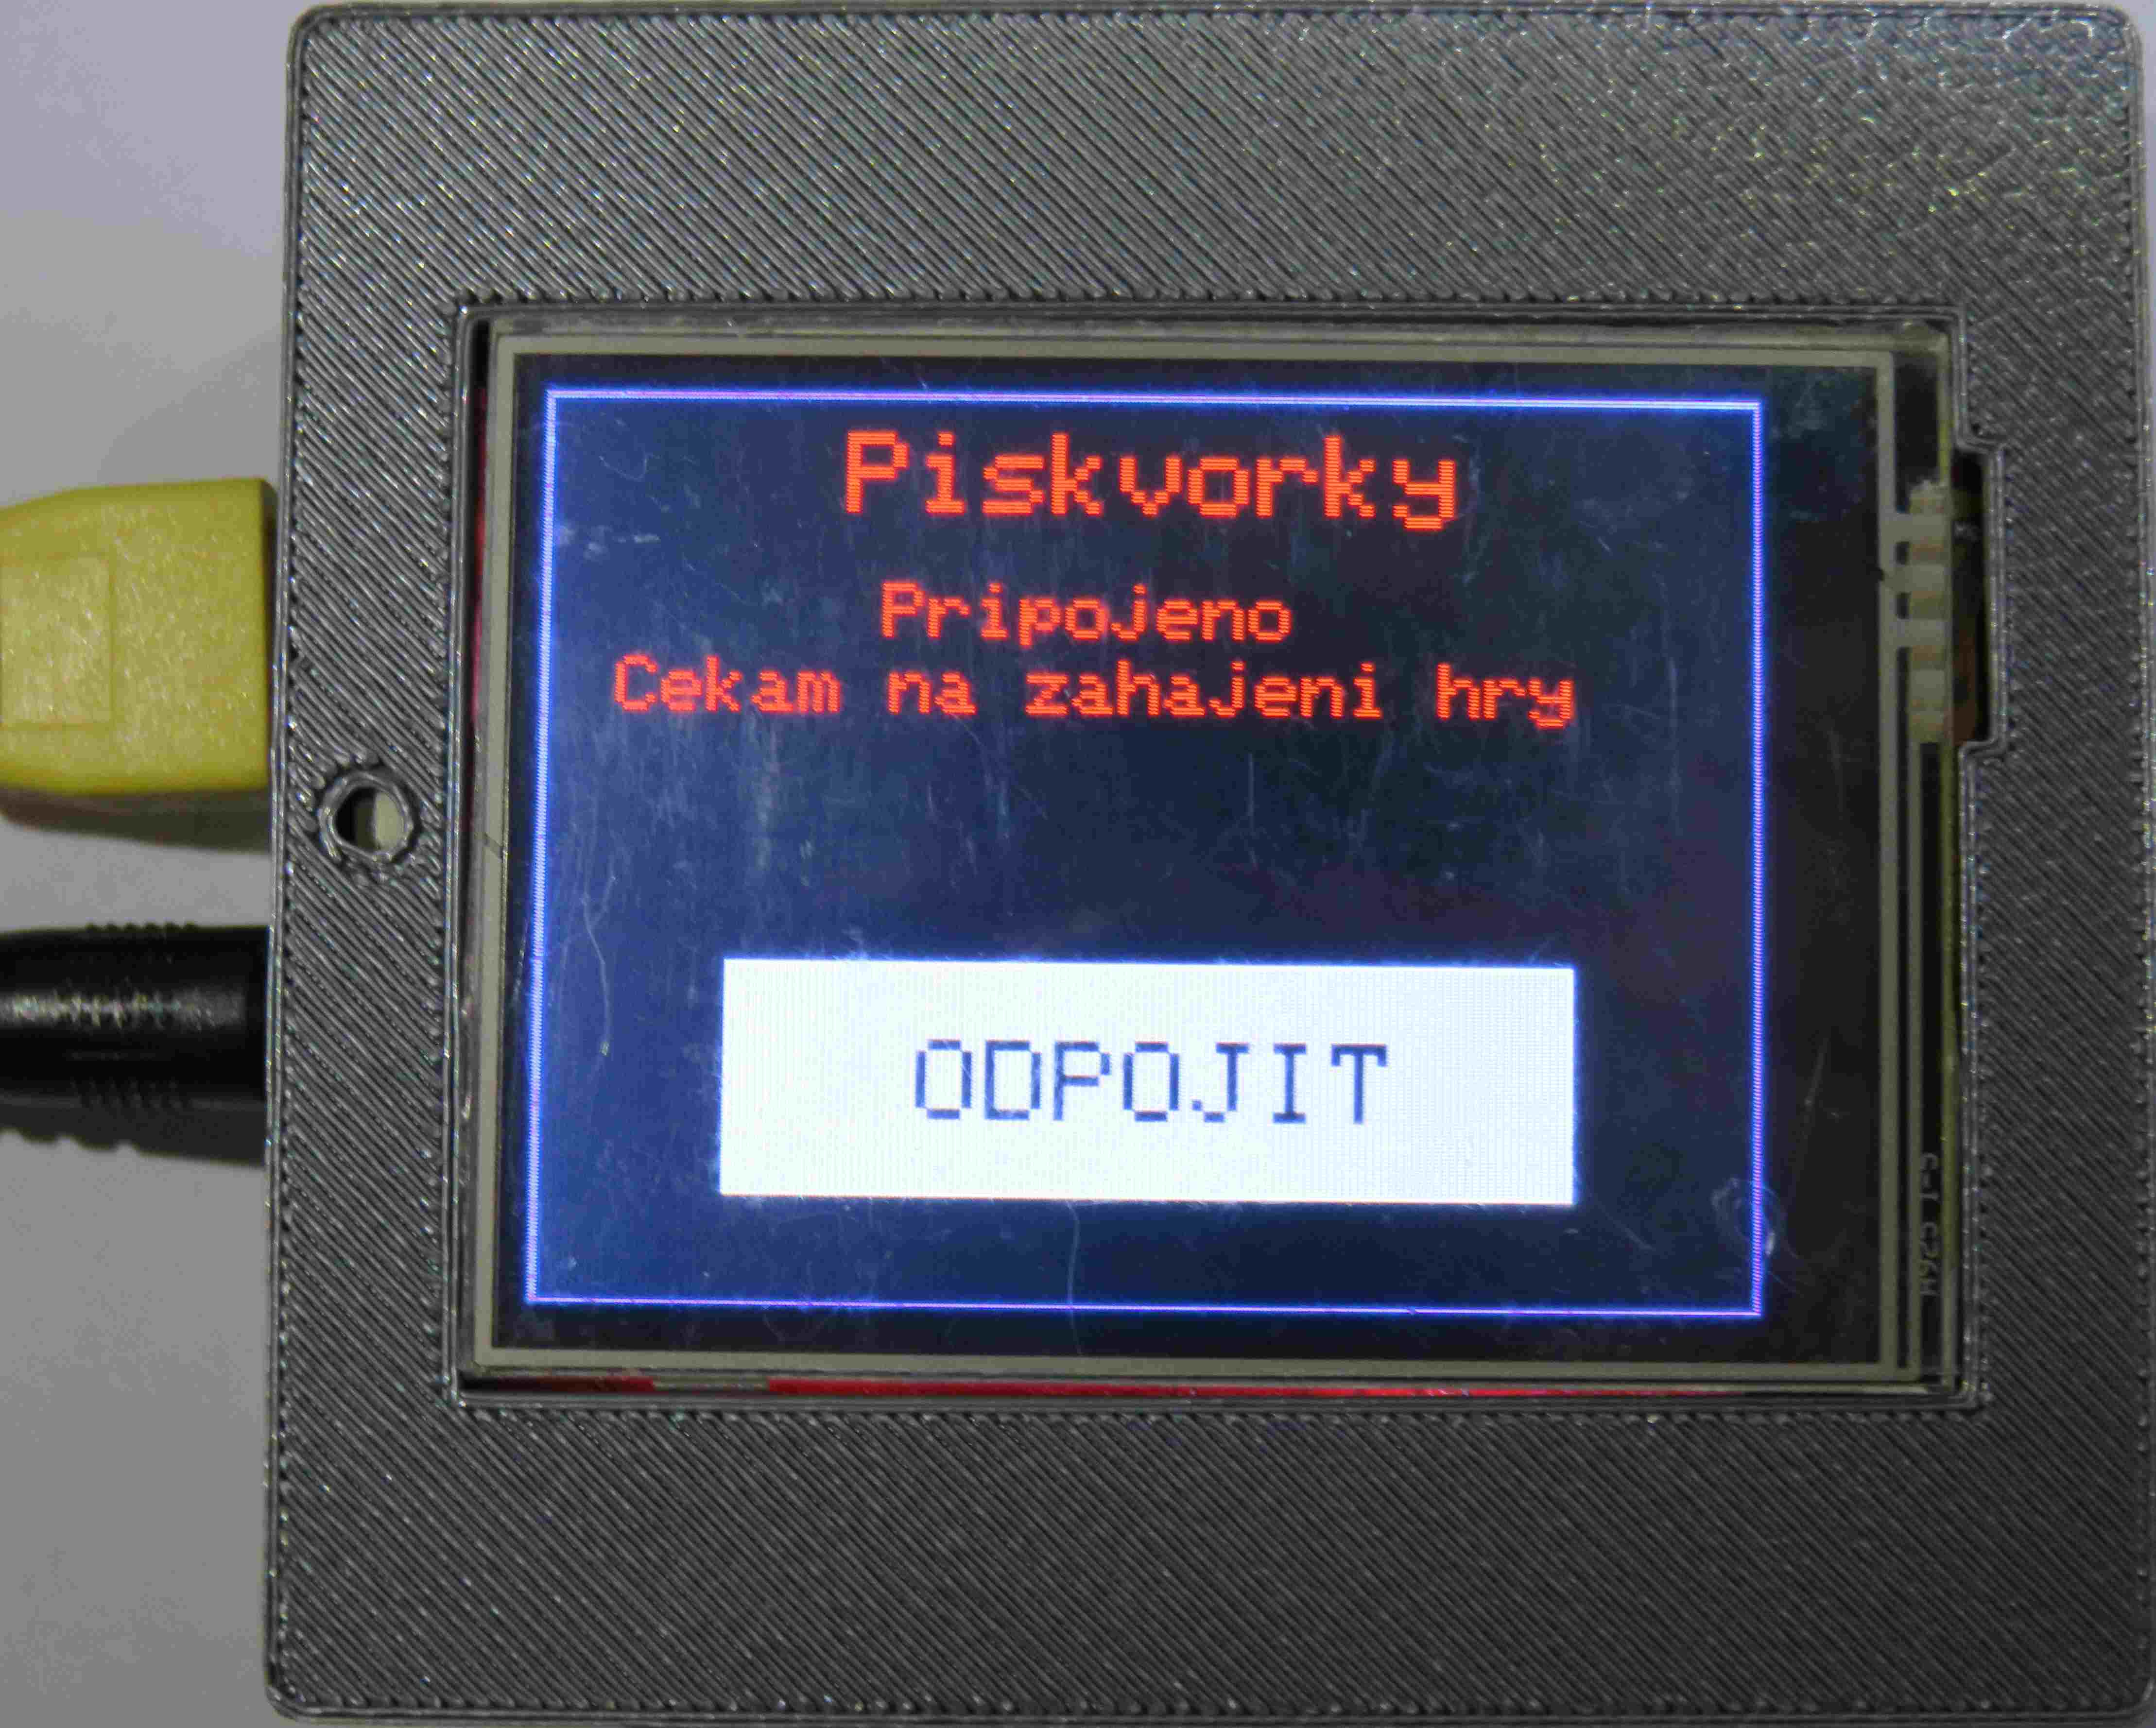
\includegraphics[width=7cm, angle=0]{img/gameFlow/phase03a.jpg}
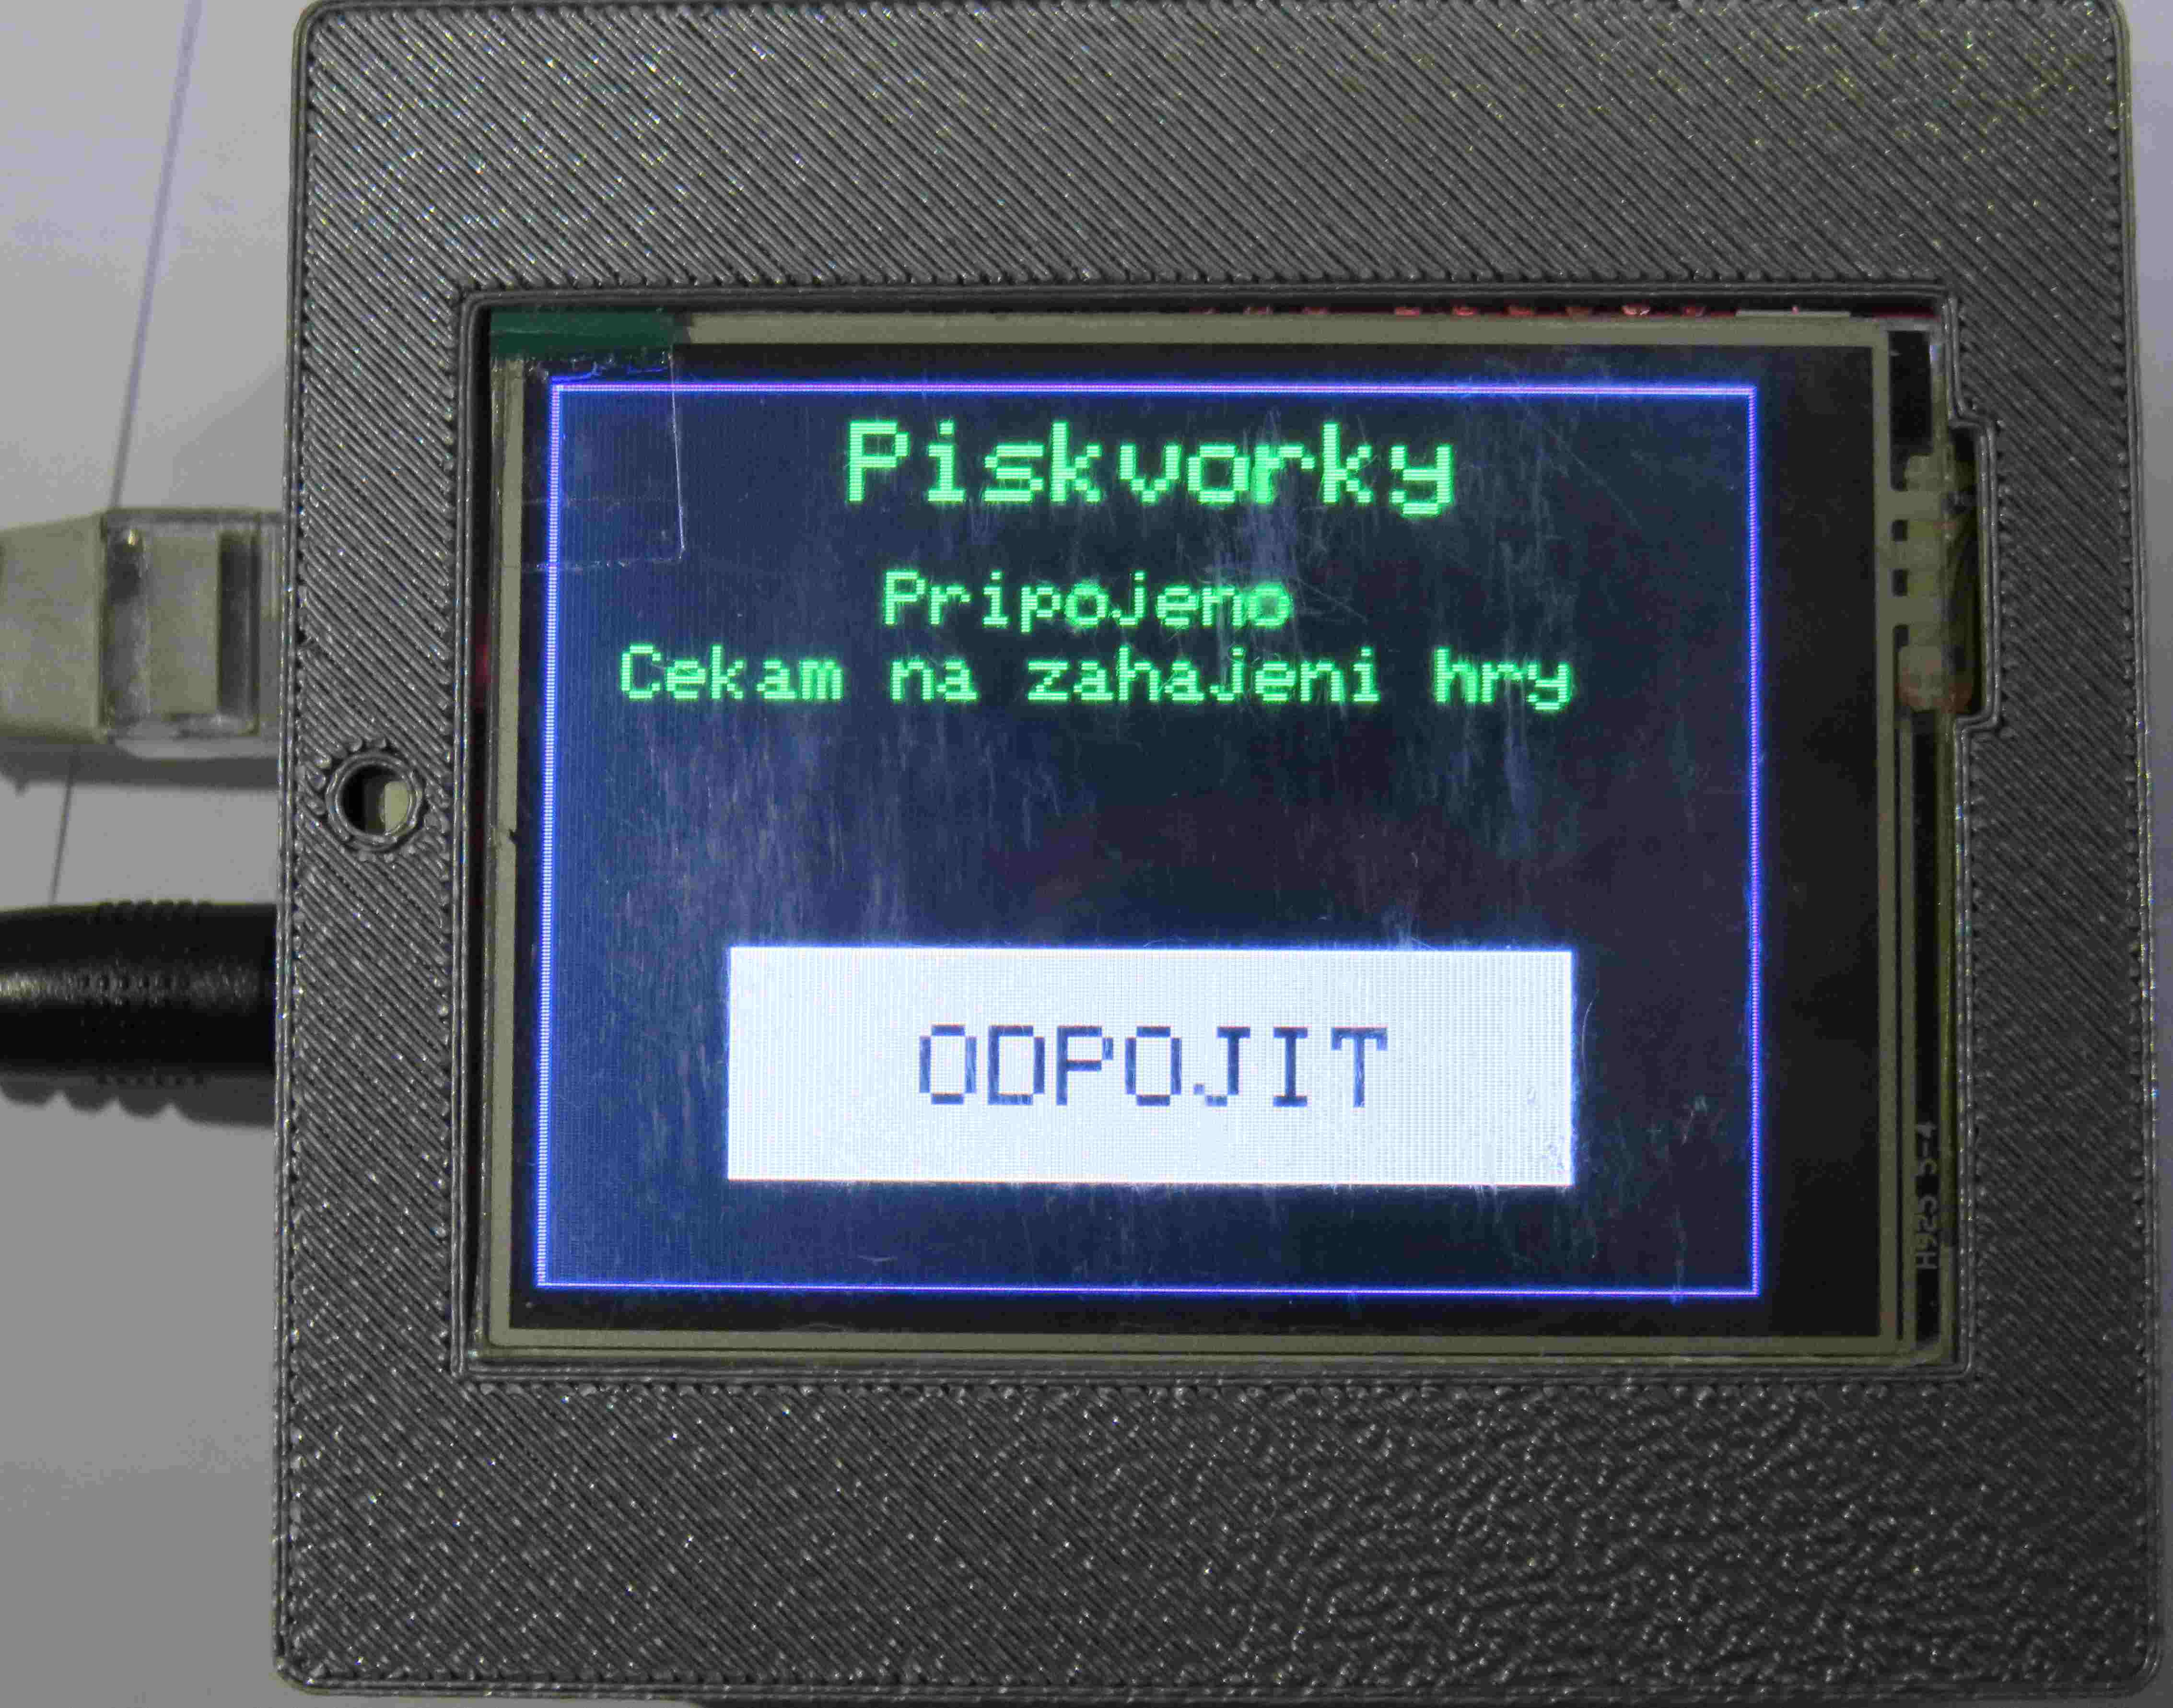
\includegraphics[width=7cm, angle=0]{img/gameFlow/phase03b.jpg}
\caption{\label{fig:faze3} Obrazovky dvou různých klientů  po úspěšném připojení k piškvorkovému serveru}
\end{figure}
\label{item:faze3}

%%%
\item V případě, že ze strany serveru byla započata hra (příkazem nebo stiskem zeleného tlačítka), vykreslí se na obrazovce herní pole (obrázek~\ref{fig:faze4}).

Jednotlivé čtverce mají pro tento typ displeje fyzický rozměr přibližně 0,5x0,5~mm. Tato velikost byla zvolena proto, že je možné na takto malý displej umístit dostatečně velké pole (11x8 čtverců) a zárověň je možné jej bez problém ovládat stylusem a případně i prstem.
\begin{figure}[H]
\centering
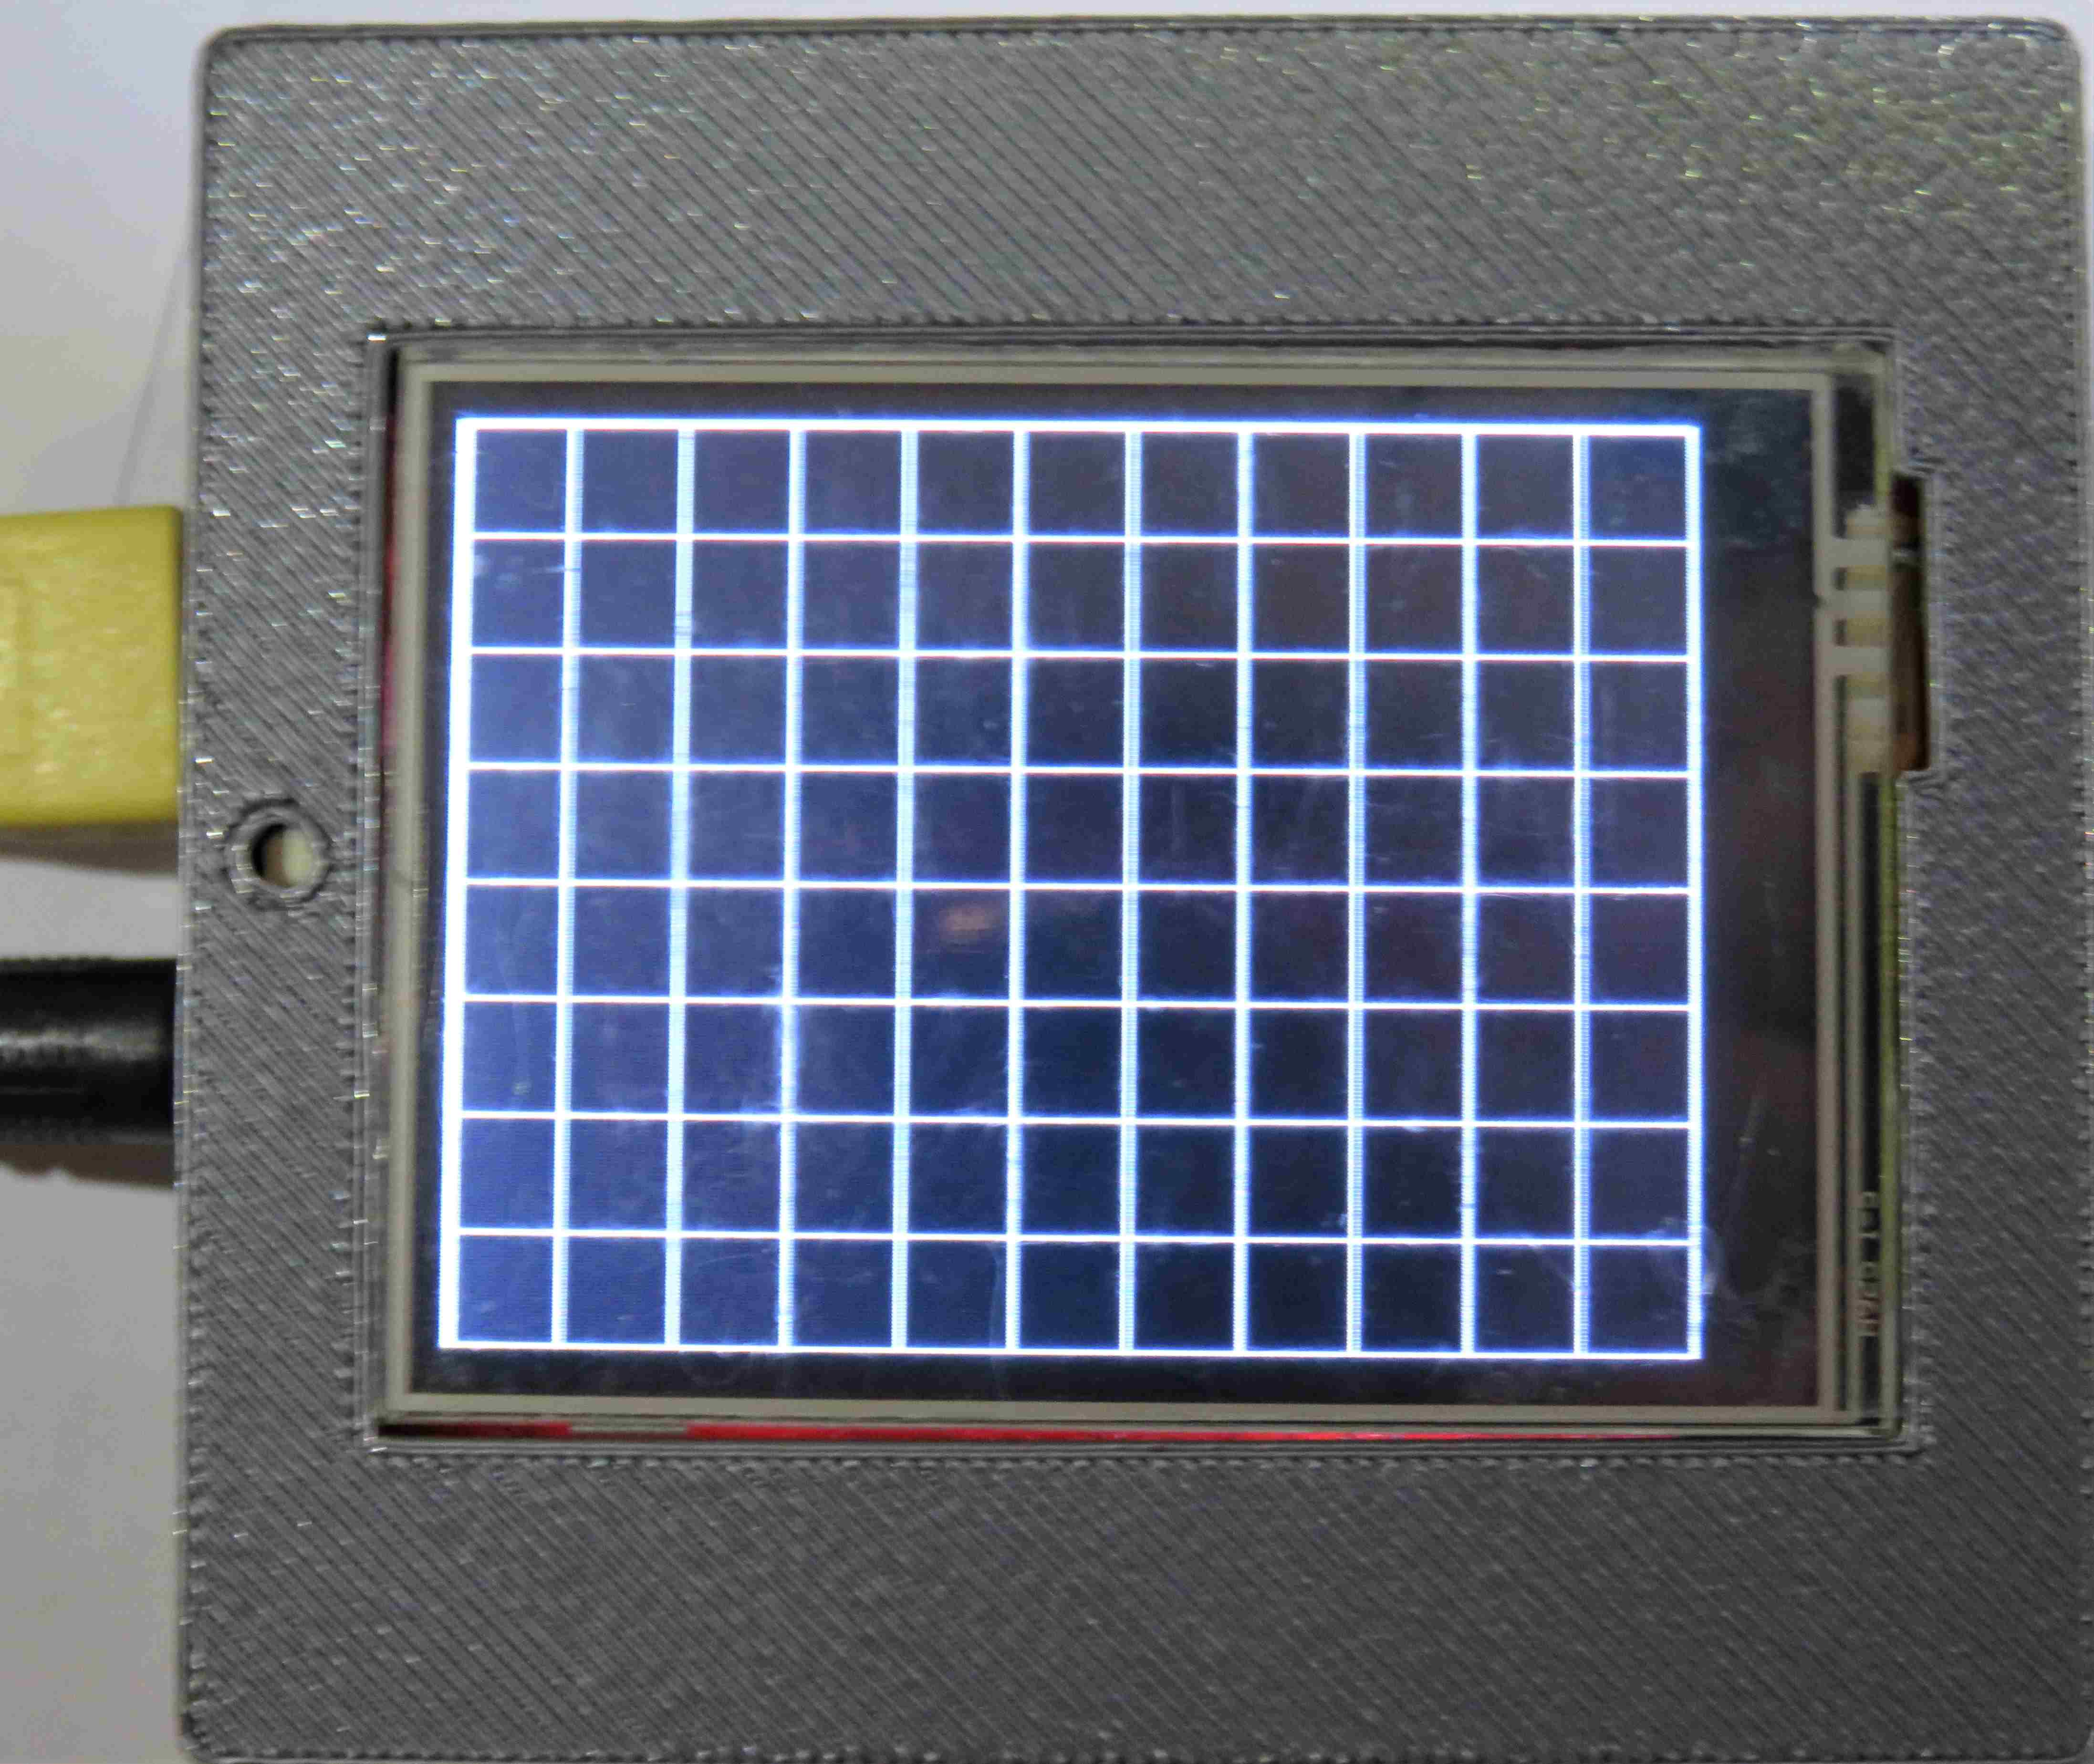
\includegraphics[width=7cm, angle=0]{img/gameFlow/phase04a.jpg}
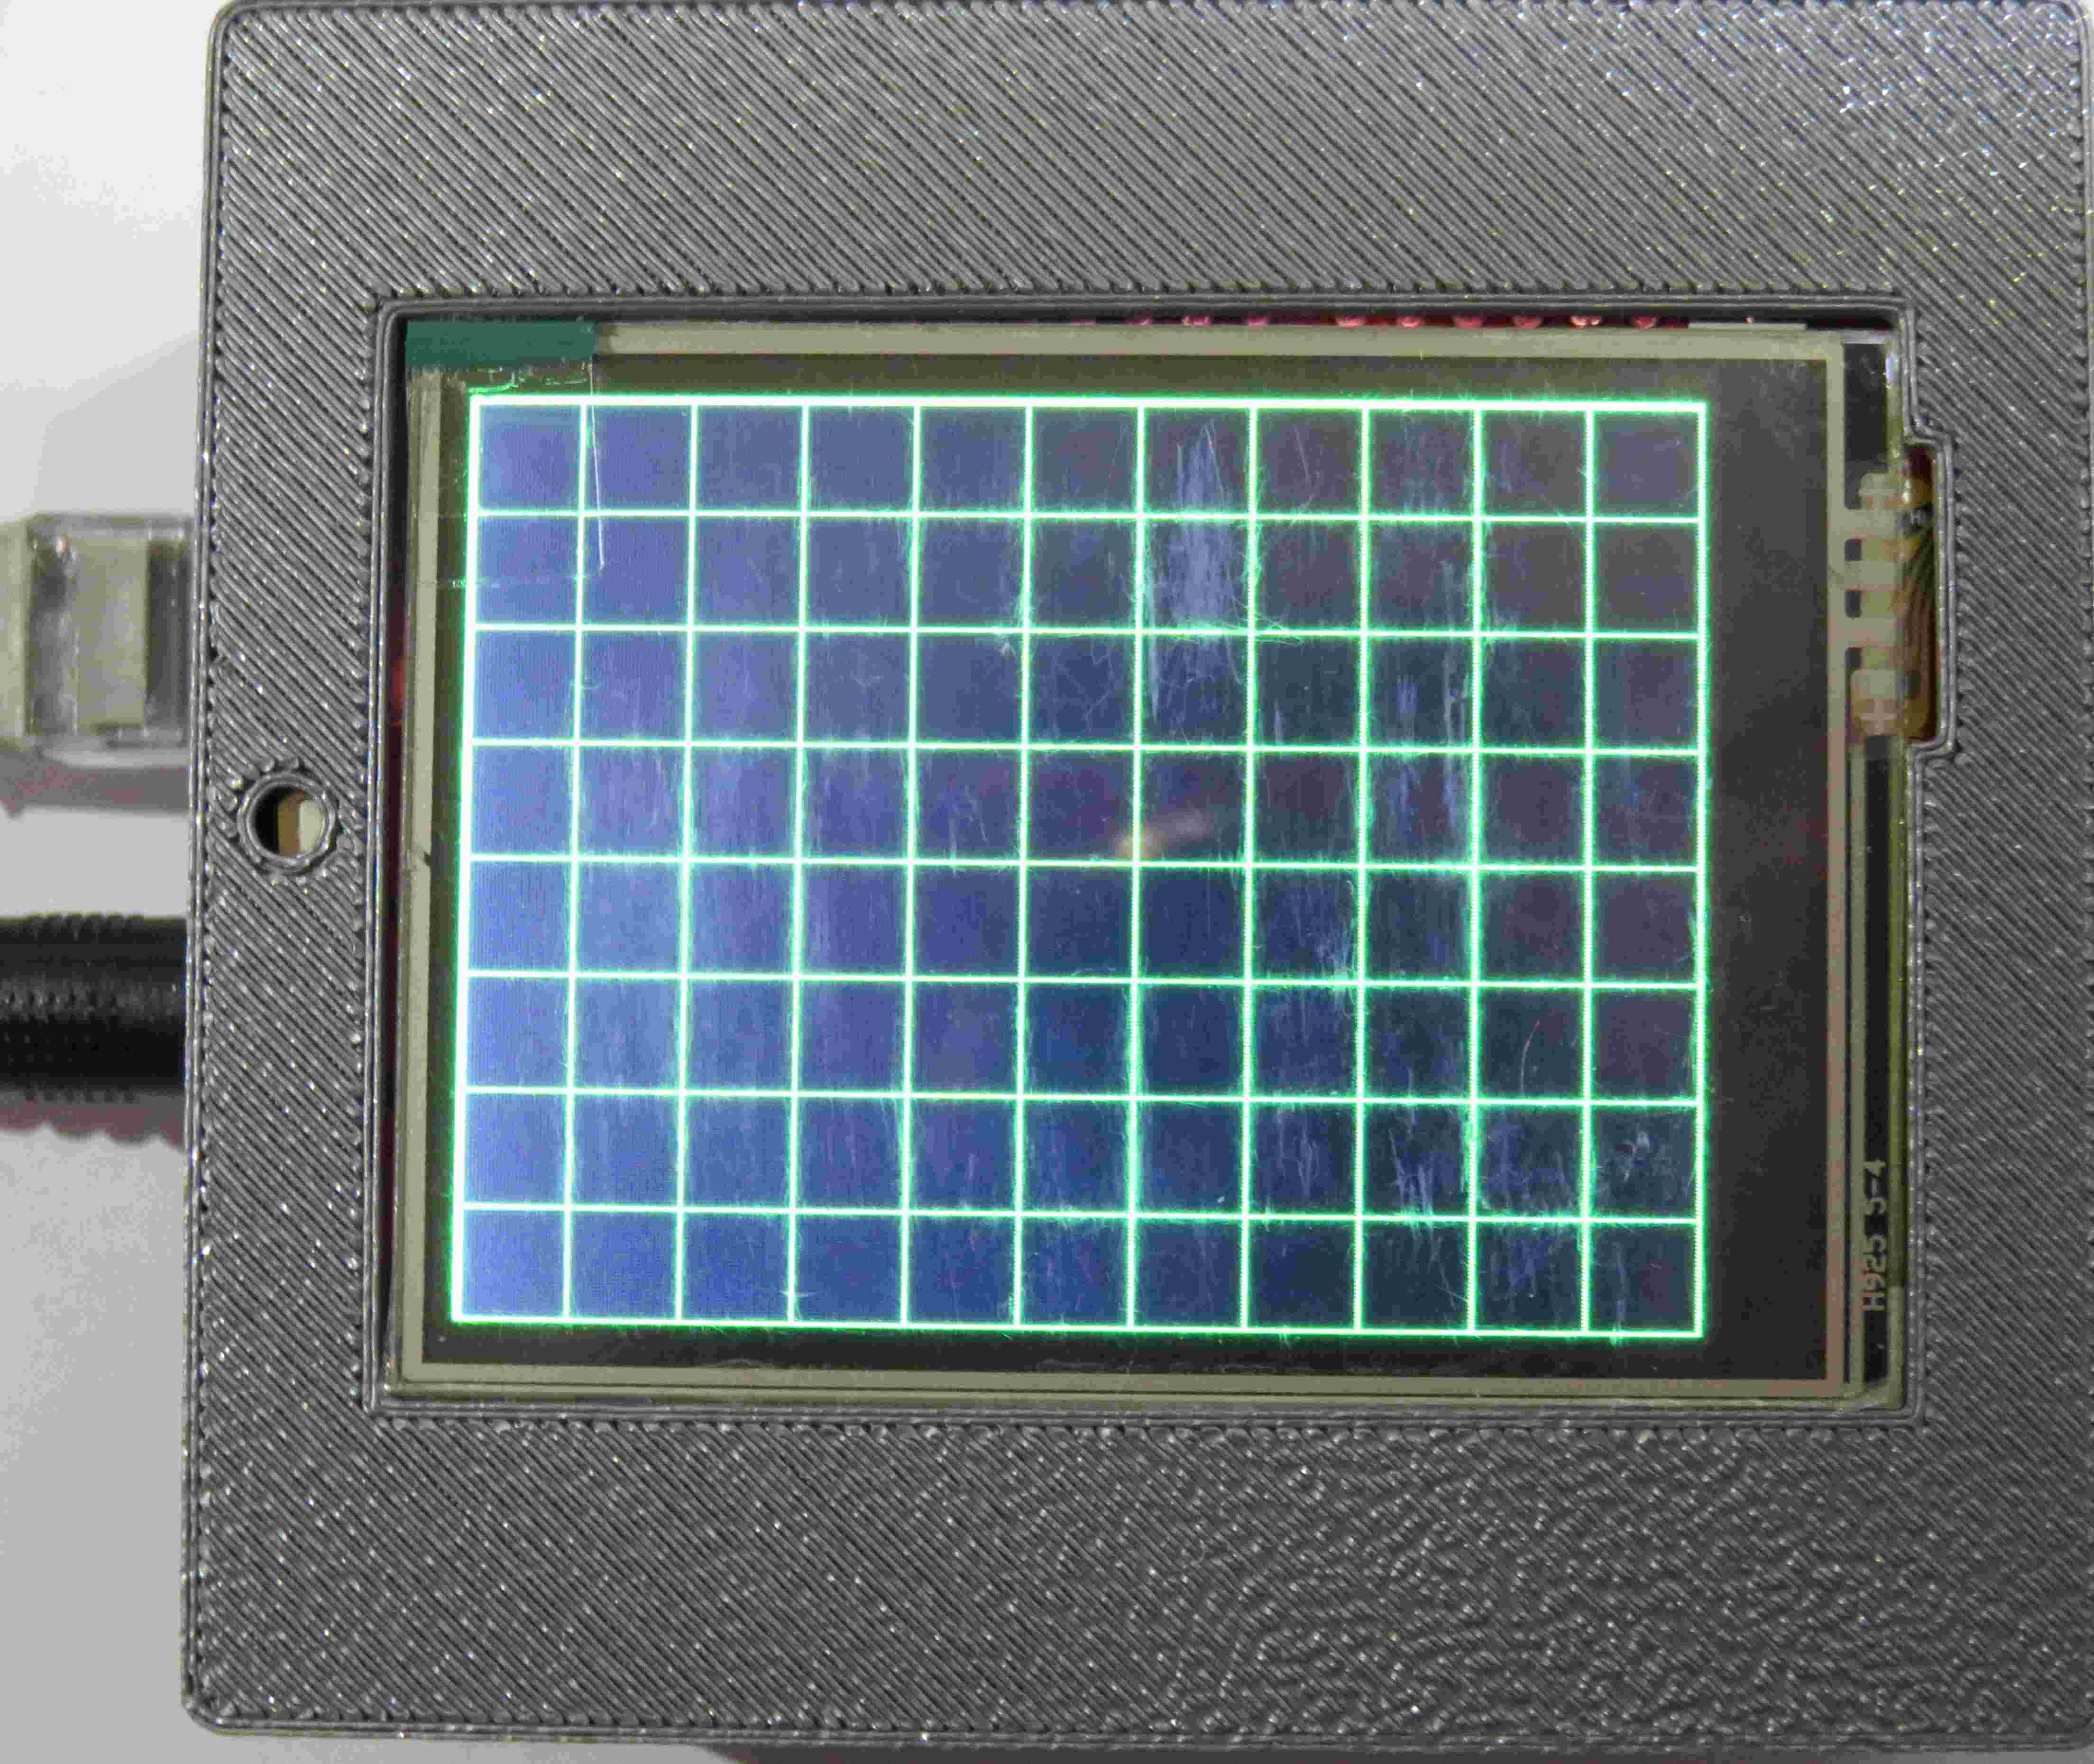
\includegraphics[width=7cm, angle=0]{img/gameFlow/phase04b.jpg}
\caption{\label{fig:faze4} Obrazovka klienta po započaté hře (a) čekající hráč, (b) hrající hráč}
\end{figure}

%%
\item Během hry: pokud je mřížky šedá, hraje jiný hráč, pokud má mřížka nějakou barvu (barva se shoduje s barvou hráče) je na tahu daný hráč. Ten má za úkol stiskem libovolného volného čtverečku umístit svůj žeton.

Když uživatel stiskne čtverec, dojde k jeho vyplnění příslušným žetonem (barevným kruhem), mříž zešedne a je na řadě další hráč. Rozehraná hra je vidět na obrázku~\ref{fig:faze5}.
\begin{figure}[H]
\centering
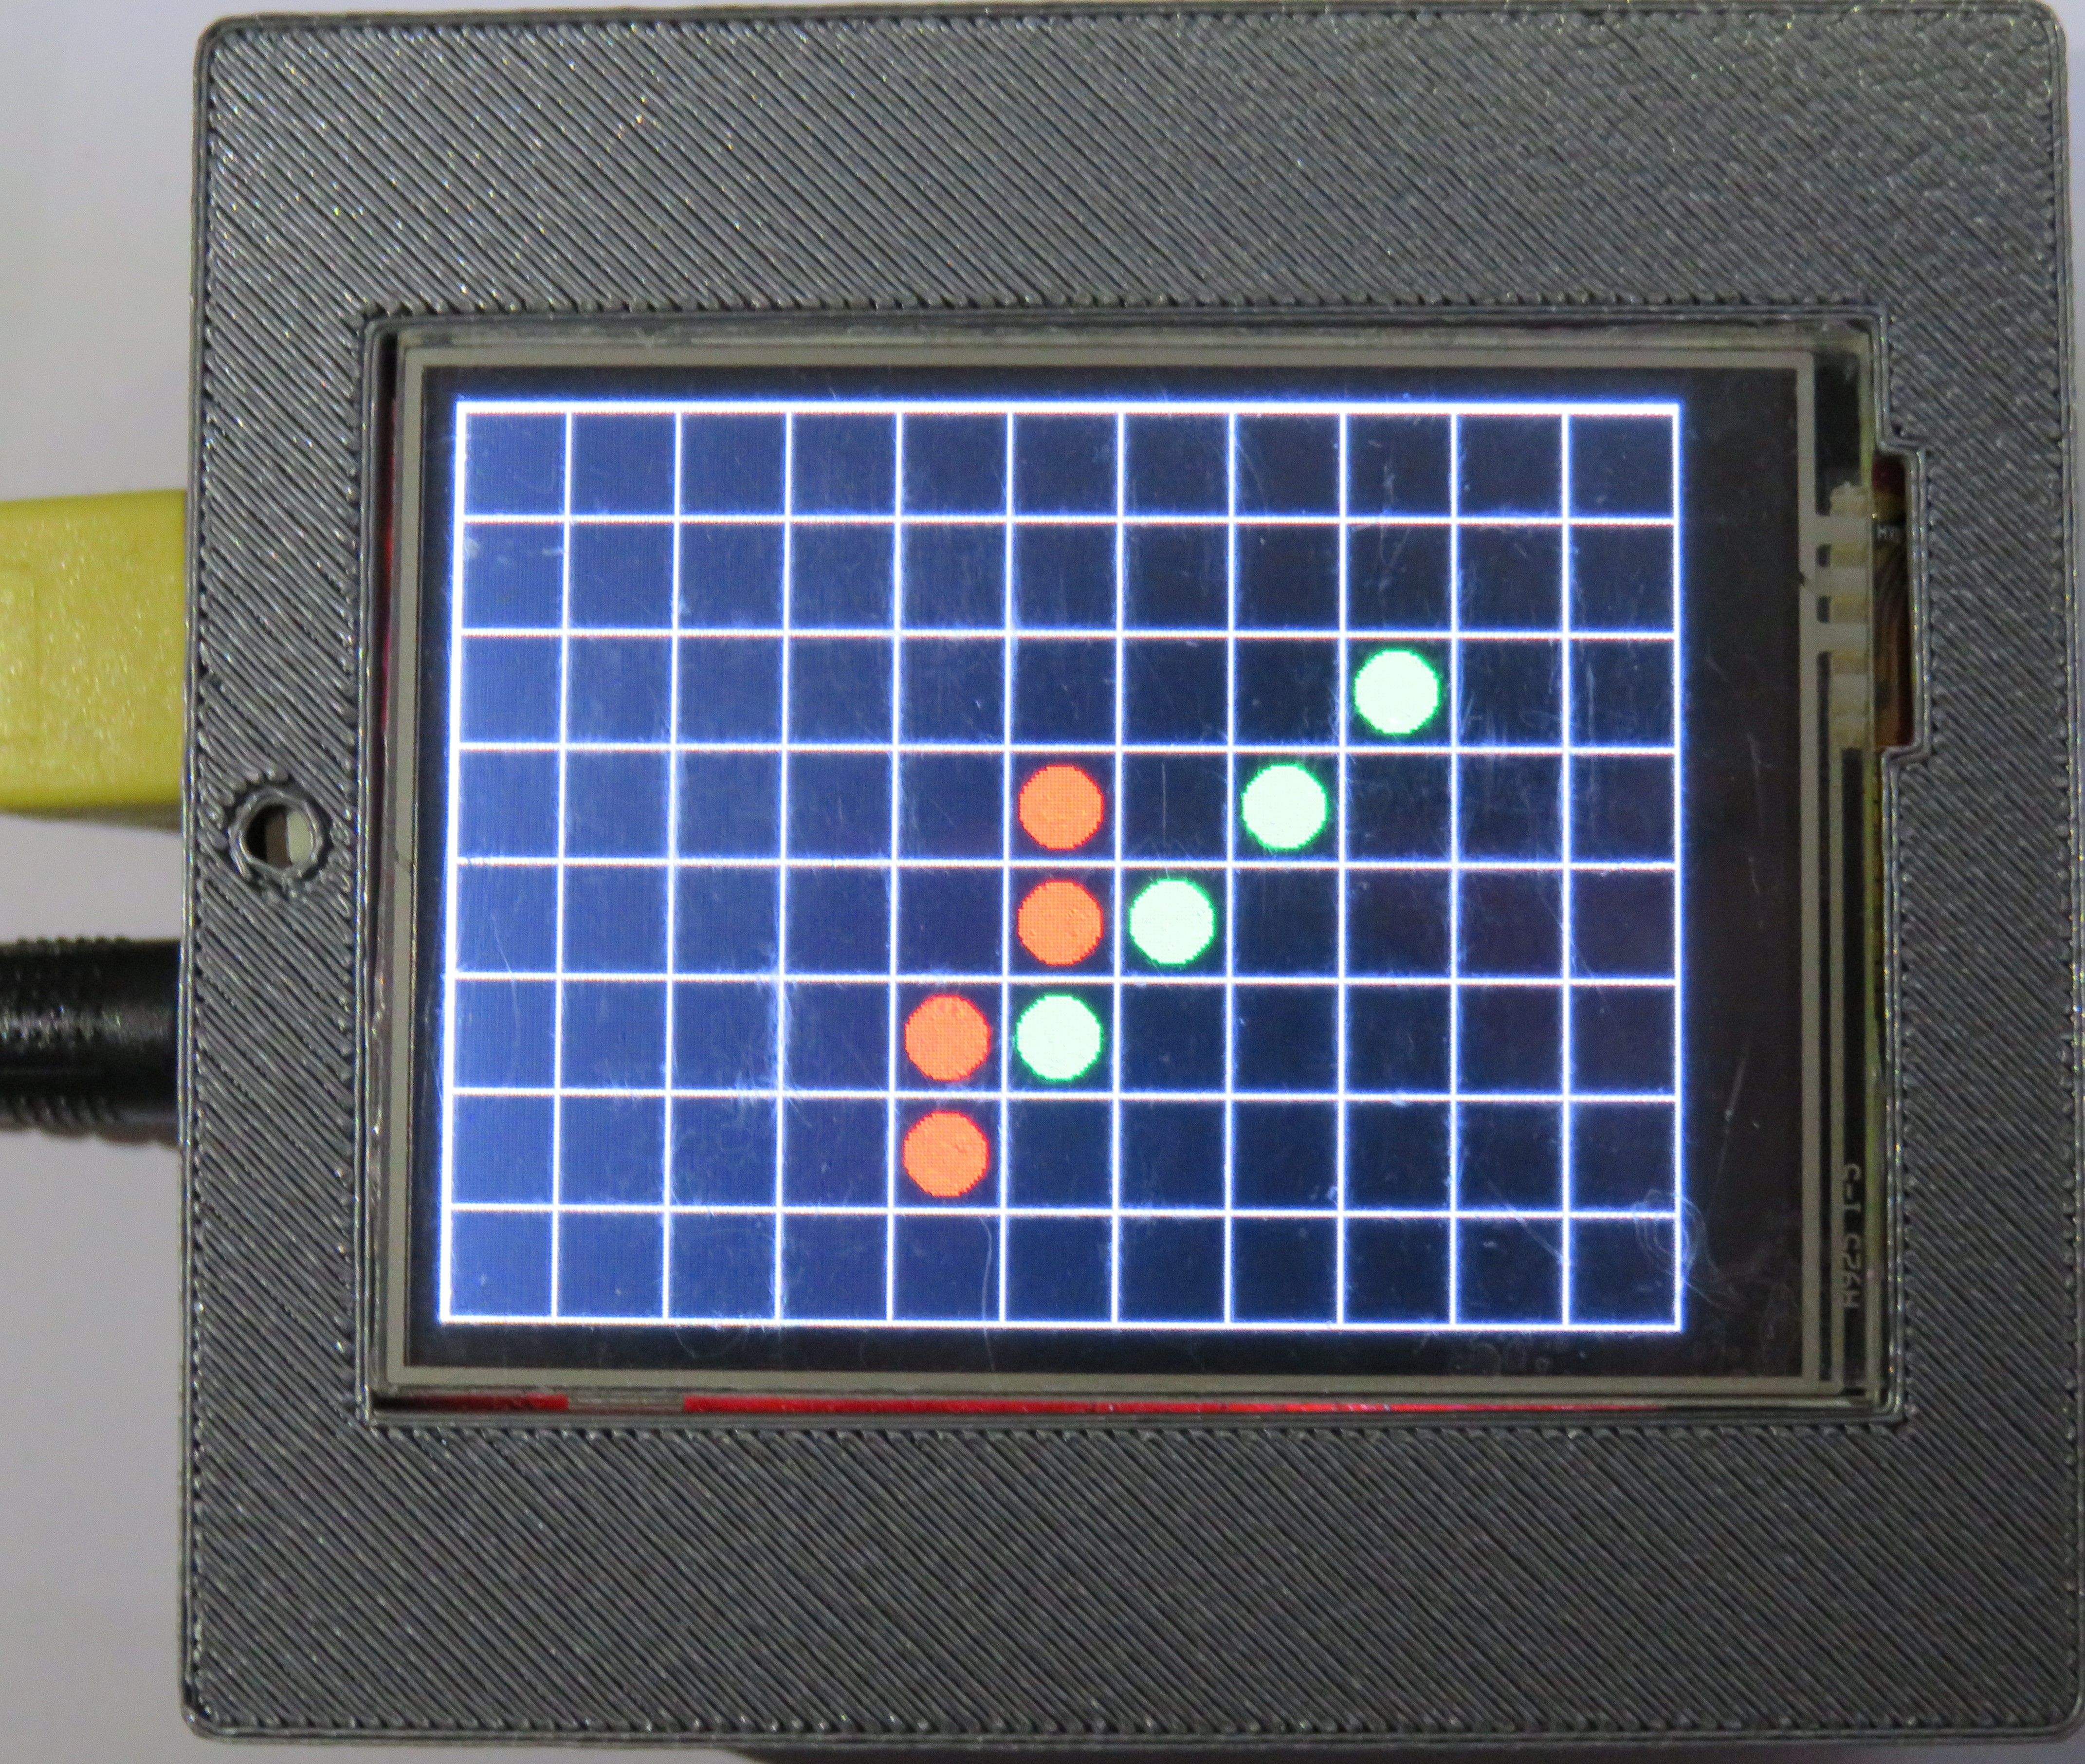
\includegraphics[width=7cm, angle=0]{img/gameFlow/phase05a.jpg}
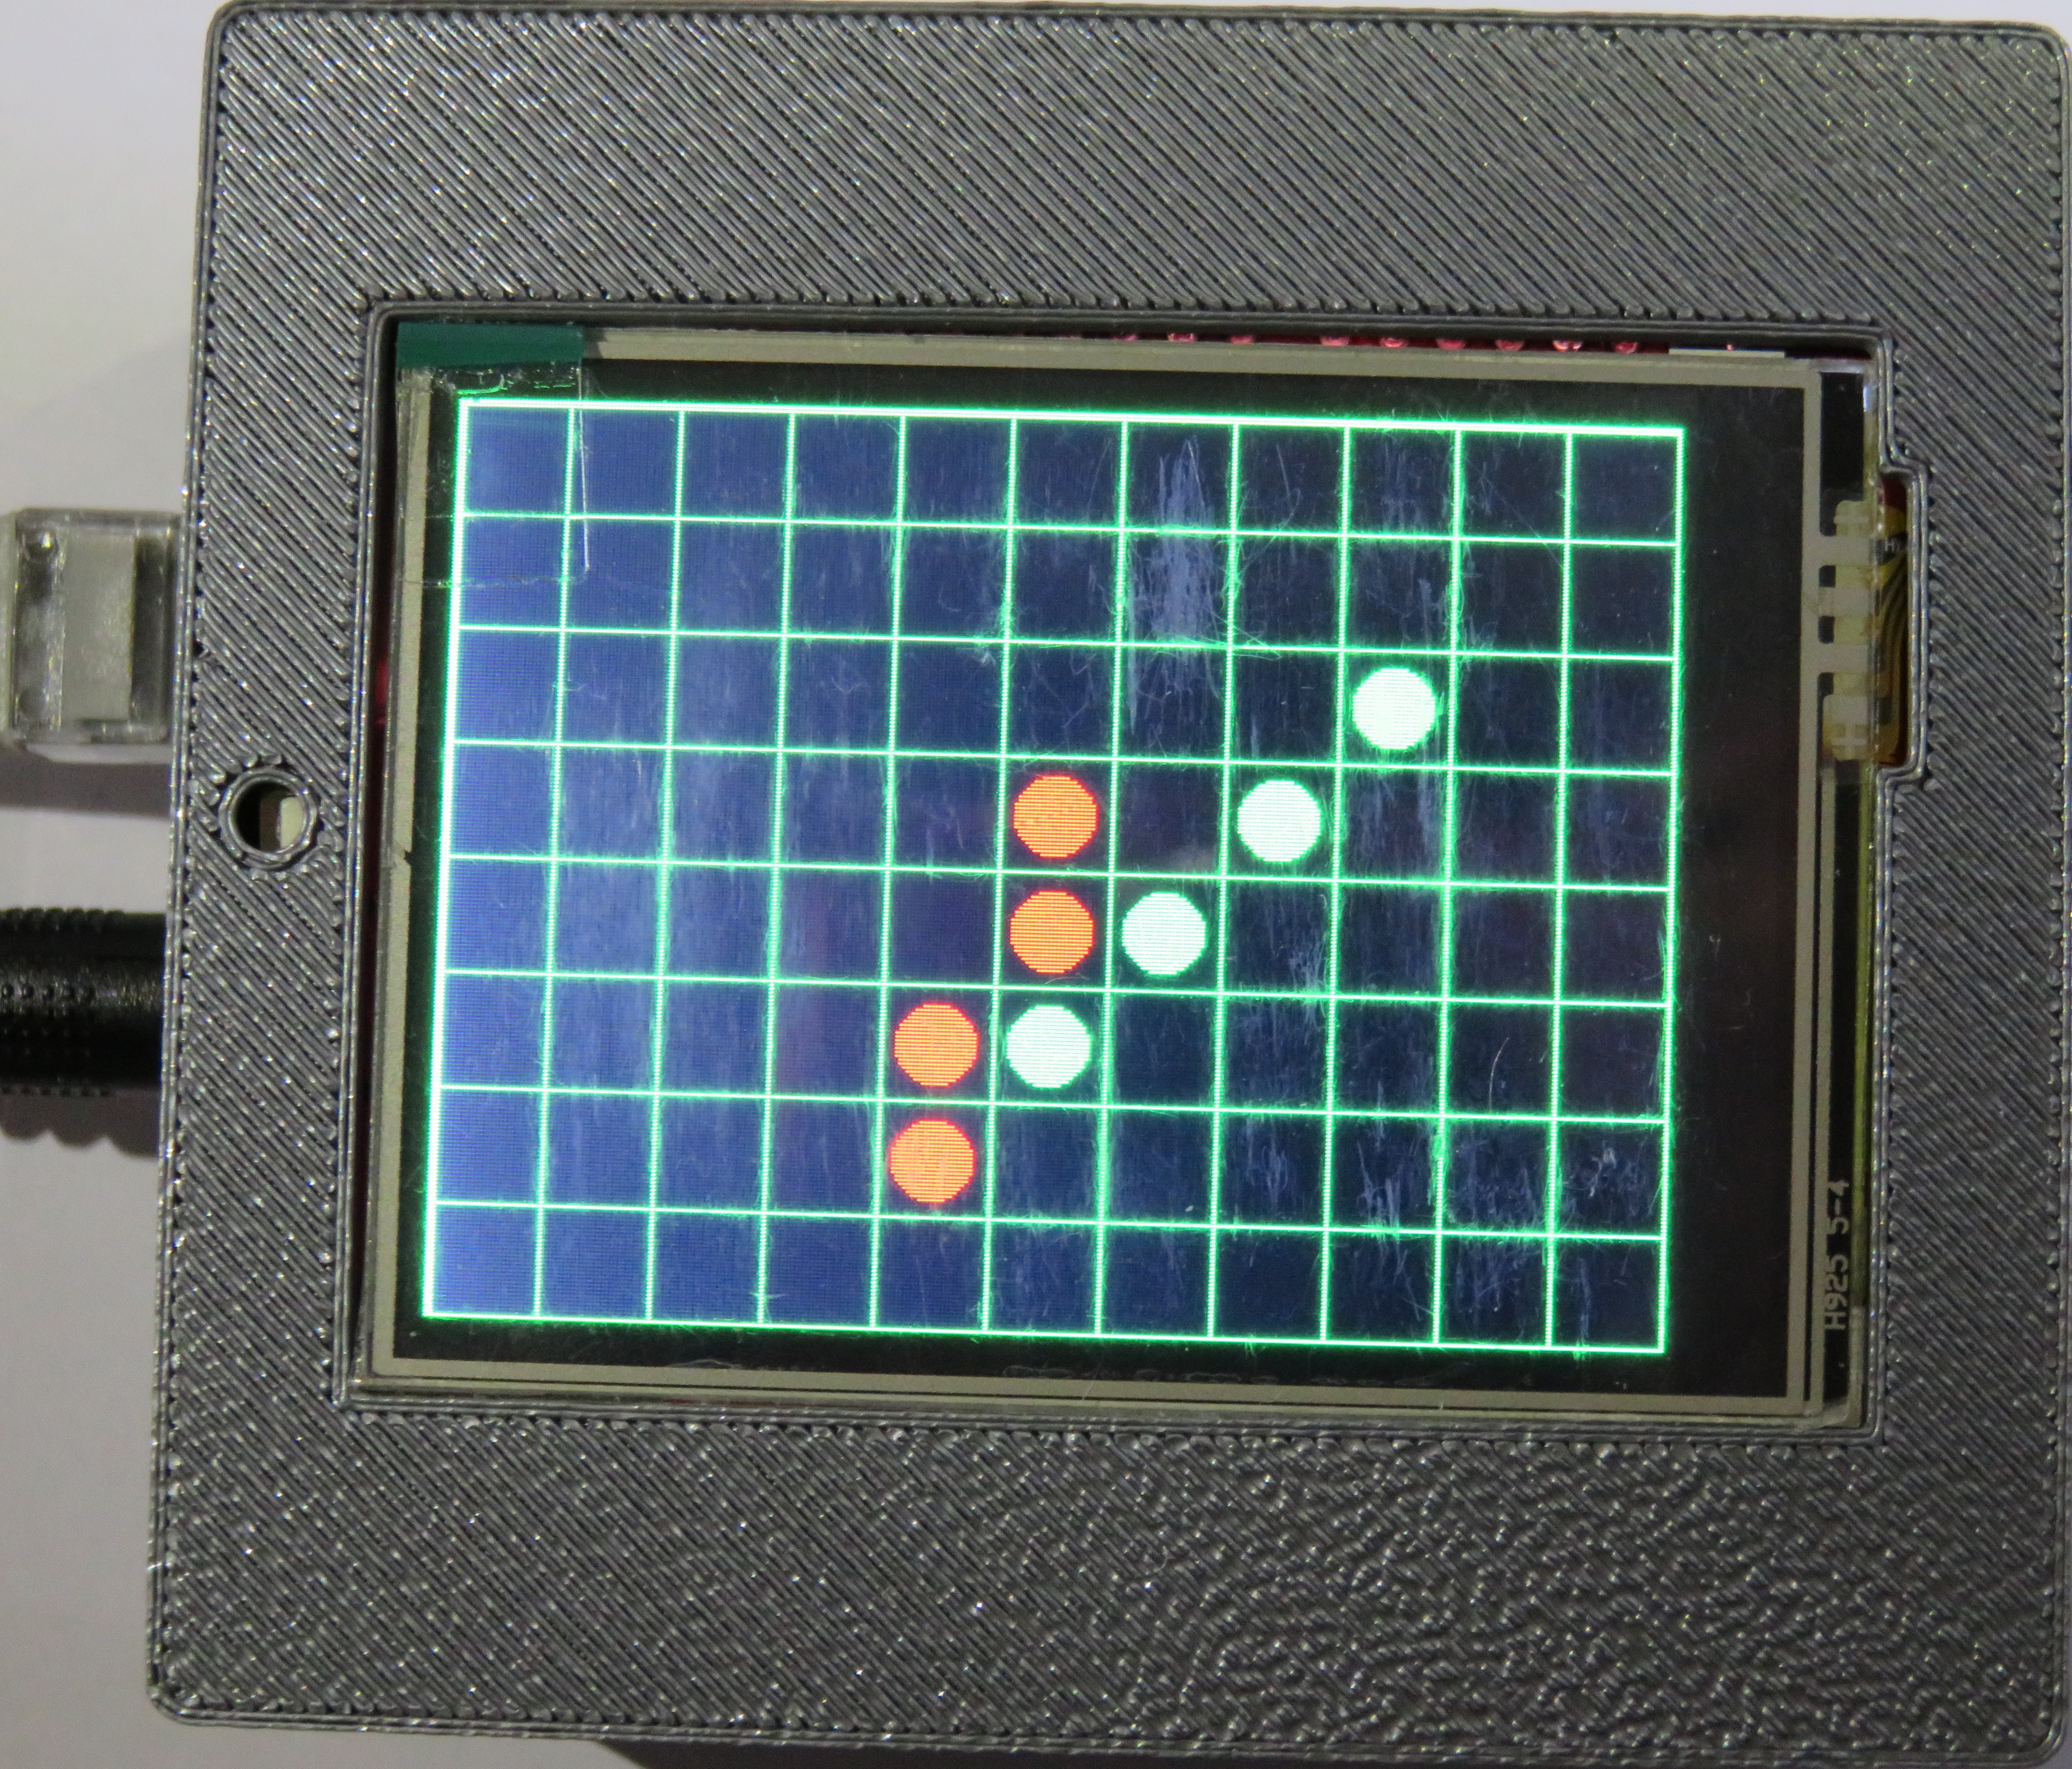
\includegraphics[width=7cm, angle=0]{img/gameFlow/phase05b.jpg}
\caption{\label{fig:faze5} Rozehraná hra dvou hráčů}
\end{figure}

%%
\item Hráči se střídají do té doby než: jsou všechna pole vyplněna (ukončeno remízou) nebo některý hráč spojil požadovaný počet žetonů (v základní nastavení pět). O výsledku hry jsou hráči informováni hláškou na displeji (obrázek~\ref{fig:faze6}). Tato hláška po deseti sekundách zmizí (nastaveno v proměnné \texttt{clientMessageLast} v milisekundách) a hra přechází do fáze~3.
\begin{figure}[H]
\centering
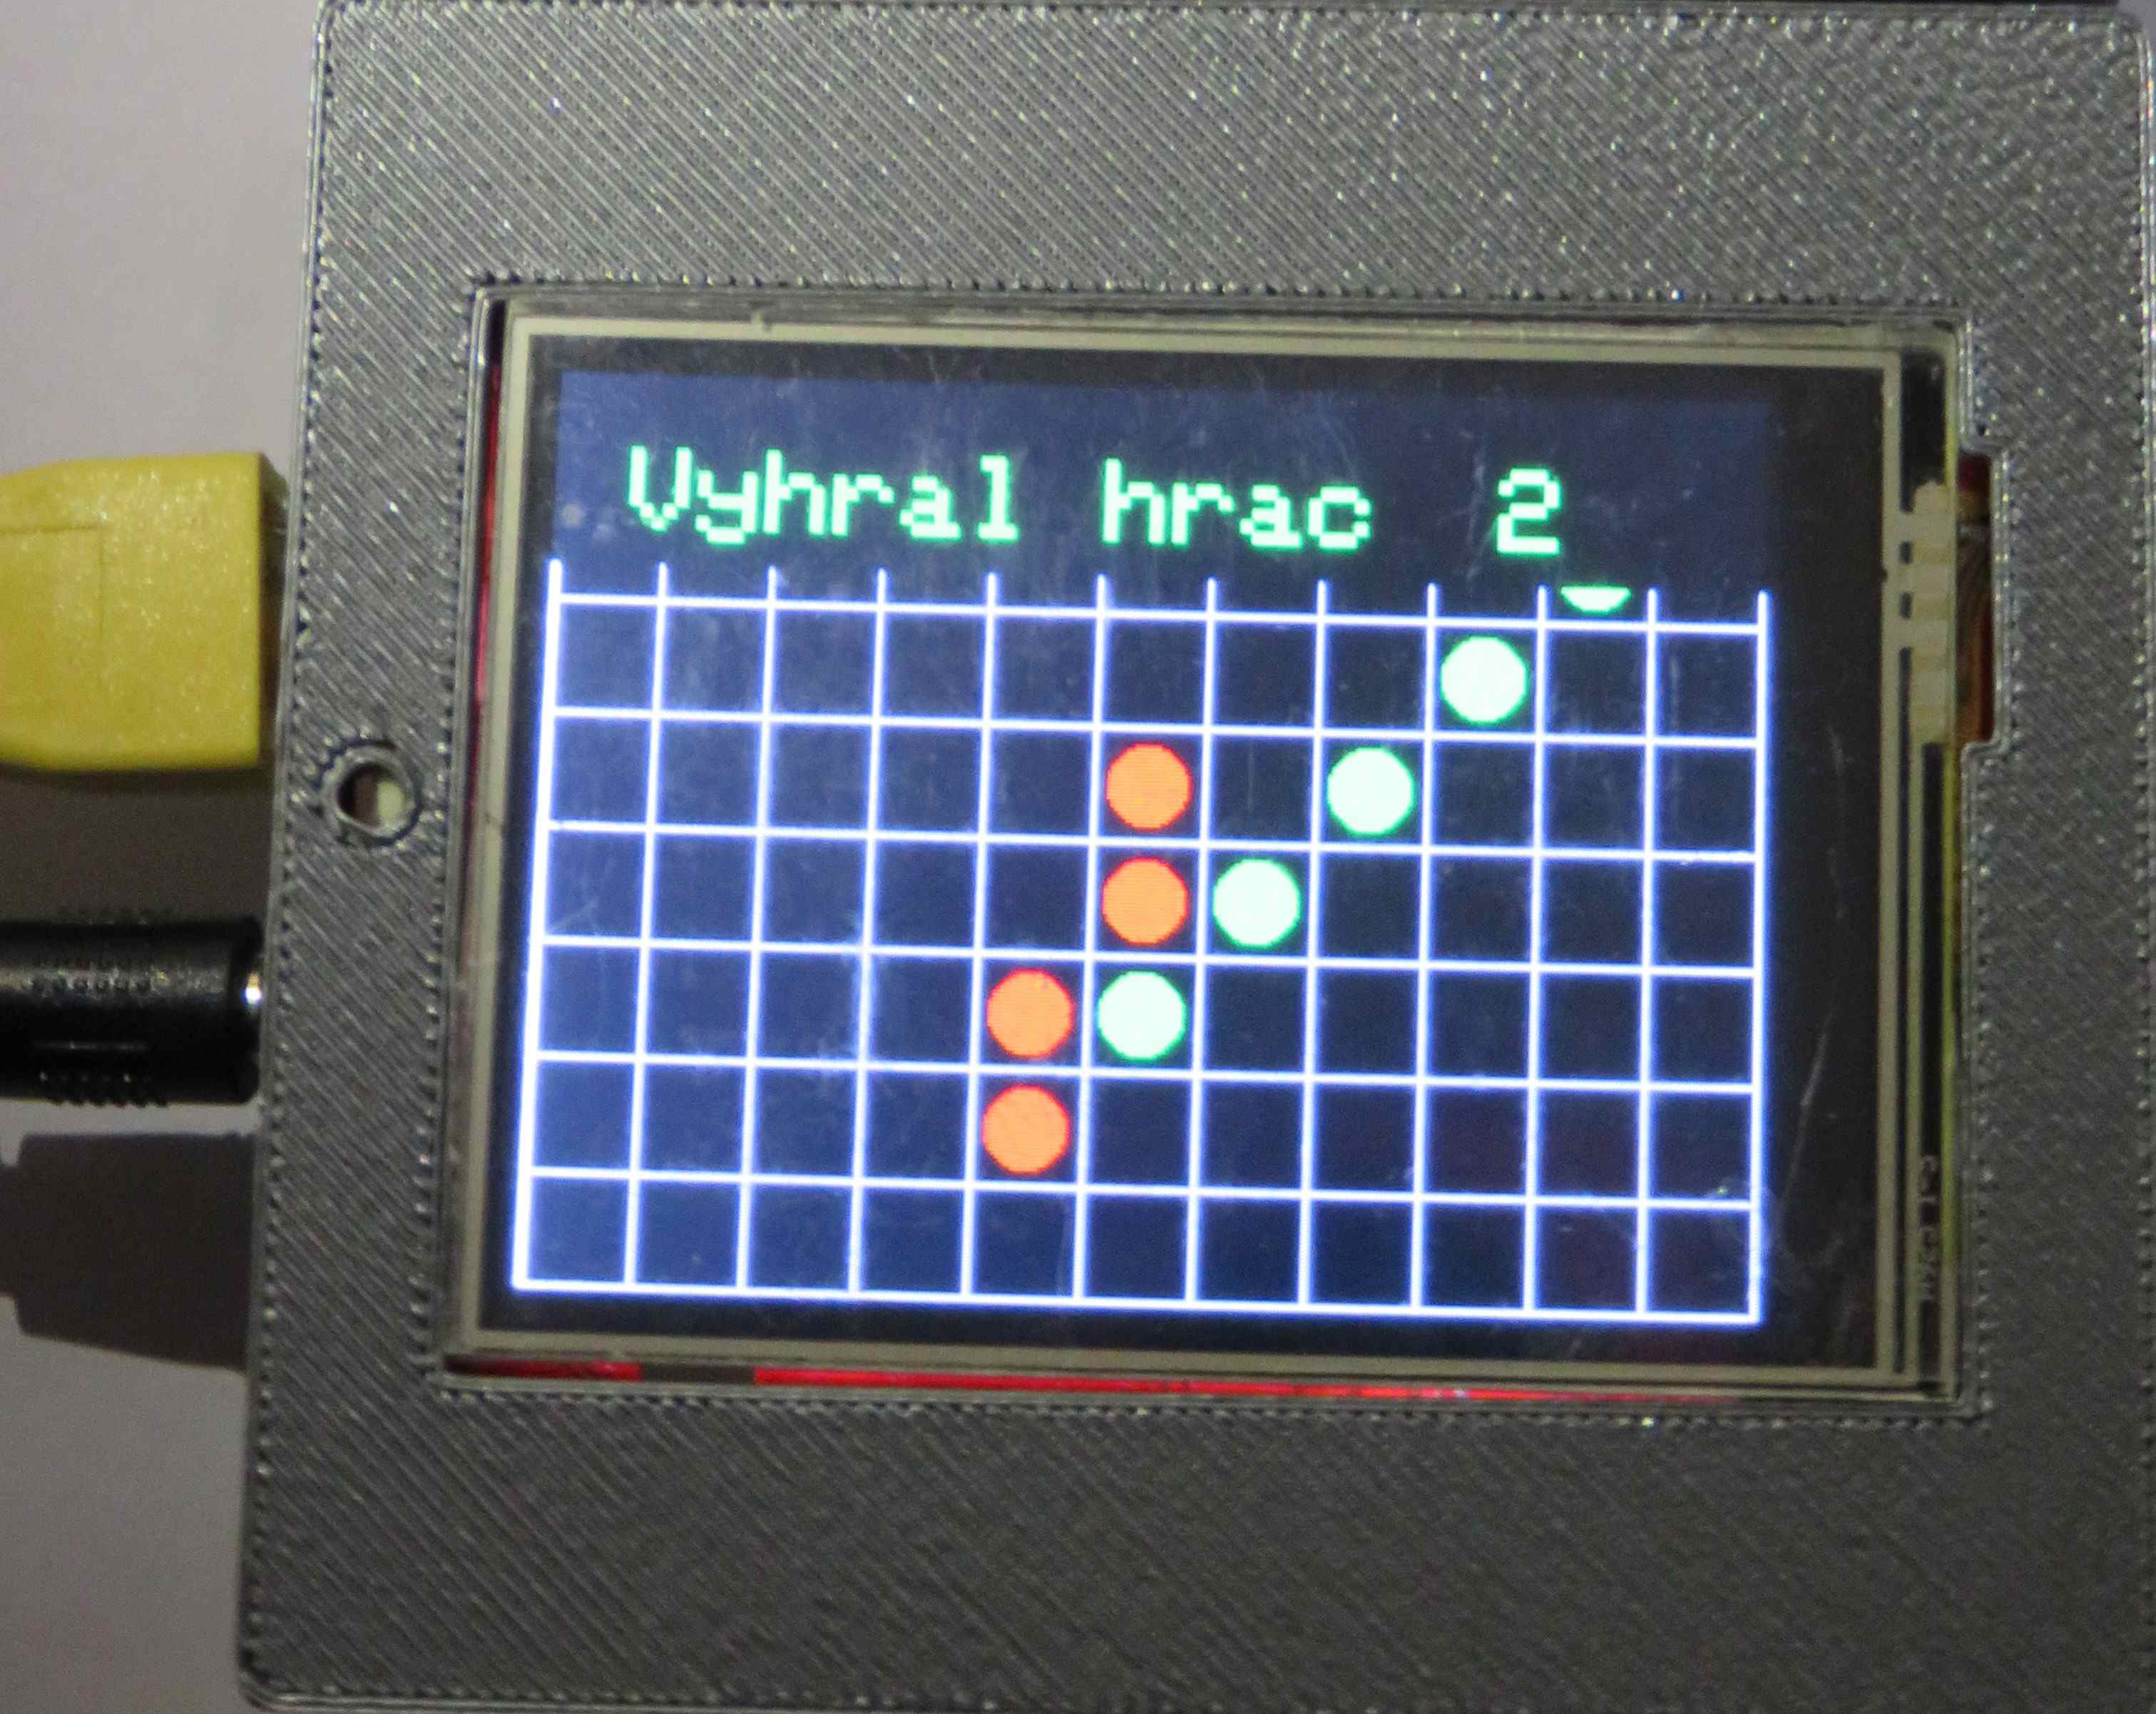
\includegraphics[width=7cm, angle=0]{img/gameFlow/phase06a.jpg}
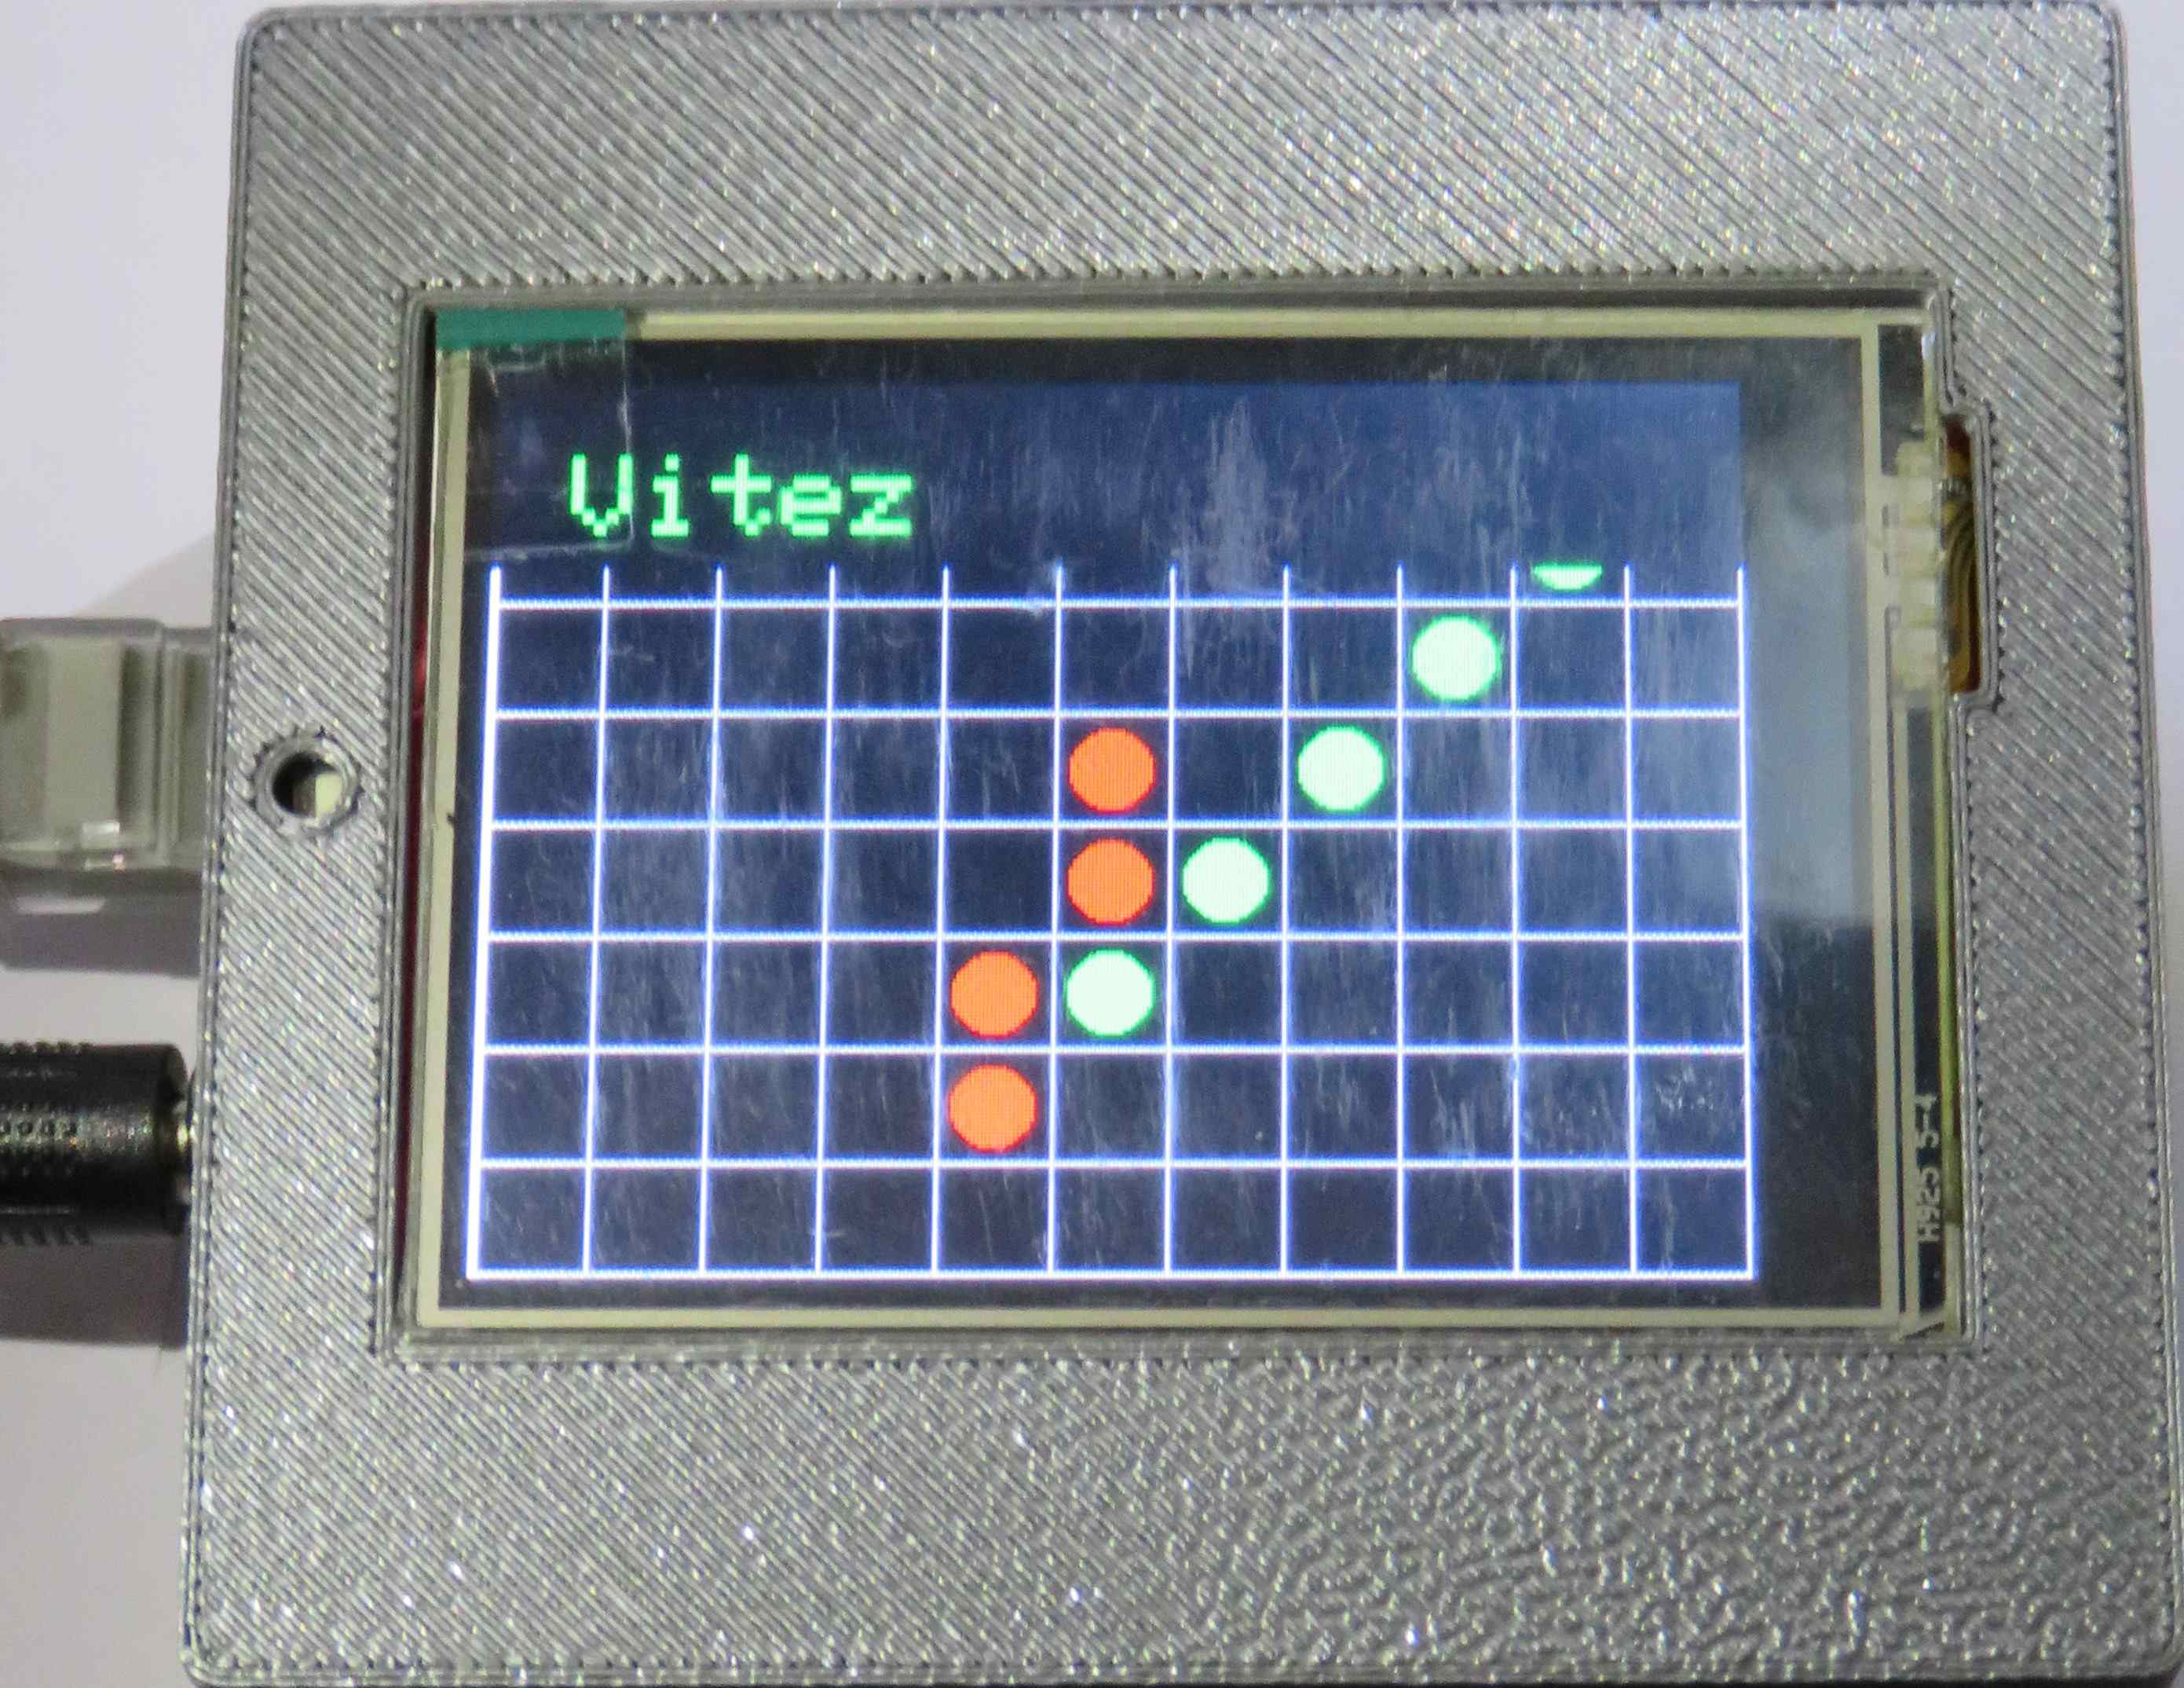
\includegraphics[width=7cm, angle=0]{img/gameFlow/phase06b.jpg}
\caption{\label{fig:faze6} Zobrazená hláška na displeji výherce (a) a ostatních hráčů (b), barva textu se shoduje s barvou vítězného hráče}
\end{figure}
\end{enumerate}
%\notFinished
\subsection{Ovládání serveru}
Server lze ovládat dvěma způsoby. Prvním z nich je ovládání pomocí dvou tlačítek.

Pokud je stisknuto červené tlačítko, dojde k přerušení hry aktuálně běžící hry (dosavadní stav hry je resetován).

Pokud je stisknuto zelené tlačítko a neběží hra (indikační LED svítí modře) - stiskem tlačítka dojde ke spuštění hry (s ověřením zda je k dispozici dostatek hráčů).
Pokud hra již běží (indikační LED svítí zeleně) stiskem zeleného tlačítka dojde k posunutí tahu na dalšího hráče.

Druhým způsobem ovládání je posílání příkazů přes sériovou linku. V tomto případě je nutné serverm připojit k počítači pomocí micro USB kabelu (konektor z přední strany serveru). K zobrazení dat lze použít nástorj \textit{Serial monitor} přímo v Arduino~IDE nebo například sériový terminál \textit{RealTerm \footnote{Domovská stránka: https://realterm.sourceforge.io/}}. Nastavení je následují: rychlost = 9600 baudů, Data bits = 8, Stop bits = 1, Flow control = none.  Každý příkaz musí být zakončen novým řádkem (LF). Seznam příkazů je v tabulce \ref{tab:server_prikazy}.

Informování uživatele o stavu serveru je realizovano pomocí barevné svítivé diody. Význa jednotlivých stavů je v tabulce \ref{tab:serverLED}. Symboly: 
\includegraphics[height=.4cm]{img/manual/blue.png} svítivá dioda svítí, 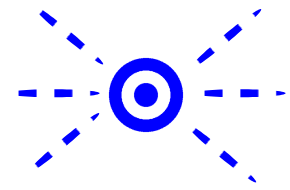
\includegraphics[height=.4cm]{img/manual/blue_blink.png} svítivá dioda bliká.

\begin{table}[hbtp]
  \centering
\caption{\label{tab:server_prikazy} Seznam příkazů dostupných pro server}
\begin{tabular}{|c|c|}
\hline
\textbf{Příkaz} & \textbf{Význam}                                        \\ \hline
help            & Vypíše nápovědu (dostupné příkazy)                     \\ \hline
info            & Vypíší informace o serveru (HW, verze SW, apod.)       \\ \hline
players         & Zobrazí čísla a IP adresy připojených hráčů            \\ \hline
kick 'x'        & Odpojí hráče číslo \textit{x}                          \\ \hline
nextP           & Přepne na dalšího hráče                                \\ \hline
start           & Spustí hru (ekvivalent zeleného tlačítka)              \\ \hline
reset           & Přeruší a resetuje hru (ekvivalent červeného tlačítka) \\ \hline
\end{tabular}
\end{table}


\begin{table}[hbtp]
\centering
\newcommand{\LEDsingHeight}{0.55cm}
\caption{Význam stavů svítivé diody na serveru, }
\label{tab:serverLED}
\label{tab:LED_man}
\begin{tabular}{|c|c|}
\hline
\textbf{Stav svítivé diody}                                            & \textbf{Význam}                  \\ \hline

\includegraphics[height=\LEDsingHeight/2]{img/manual/black.png}             & server je vypnutý/nemá napájení  \\ \hline

\includegraphics[height=\LEDsingHeight]{img/manual/blue.png}              & server je připraven              \\ \hline

\includegraphics[height=\LEDsingHeight]{img/manual/violet_blink.png} 3x   & nový klient připojen             \\ \hline

\includegraphics[height=\LEDsingHeight]{img/manual/orange_blink.png}   3x & klient se odpojil/byl odpojen    \\ \hline
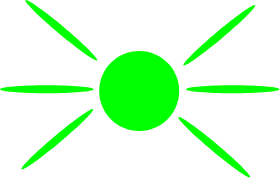
\includegraphics[height=\LEDsingHeight]{img/manual/green.png}             & aktuálně běží hra                \\ \hline

\includegraphics[height=\LEDsingHeight]{img/manual/green_blink.png}       & hra ukončena (výhra/remíza)      \\ \hline
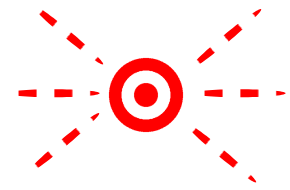
\includegraphics[height=\LEDsingHeight]{img/manual/red_blink.png} 3x      & chyba (nedostatek hráčů pro hru) \\ \hline
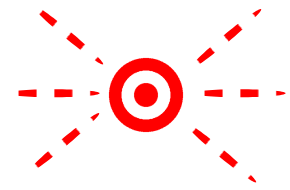
\includegraphics[height=\LEDsingHeight]{img/manual/red_blink.png} stále   & chyba sítě (připojení kabelu)    \\ \hline
\end{tabular}
\end{table}

%\notFinished

\cleardoublepage

%\setcounter{figure}{0}
%\setcounter{table}{0}
%\setcounter{equation}{0}
\section{Závěr}
V rámci této bakalářské práce se podařilo sestrojit zařízení, která zábavnou formou demonstruje možnosti komunikace nízkoenergetický jednočipových počítačů (Arduin) po síti a tím i prezentovat možnosti komunikace v IoT sítí, kdy mezi jednotlivými zařízeními není potřeba přenášet velké množství dat.

Během realizace projektu se vyskytlo několik problémů, některé z nich bylo možné úplně eliminovat, jiné vedly k určitým kompromisům. Všechny tyto problémy jsou pak zmíněny v této práci včetně zvoleného řešení. I když zařízení bylo během vývoje pravidelně testováno, nevylučuje se, že by mohlo obsahovat chyby. Opravené kódy pak~budou zveřejňovány na autorově \href{https://github.com/janzavorka/BP_PROJ}{GitHubu}\footnote{Adresa: https://github.com/janzavorka/BP\_PROJ}, kde má celý projekt od počátku vytvořenou stránku. Kromě všech zdrojových kódů, na ní lze nalézt i tuto práci a další materiály, například soubory krabiček (stl soubory i soubory pro program Autodesk Inventor). Krom oprav chyb zde budou umístěna i případná vylepšení.

\blankpage
\cleardoublepage

% \bibliographystyle{ieeetr}
% \bibliography{sample}

% \section*{Abstrakt}
Tato bakalářská práce se zabývá vývojem a výrobou jednoduchého zařízení, které umožňuje demostrovat využití energeticky nenáročných zařízení v IoT sítích. Zařízení má podobu jednoduché hry pro více hráčů - piškvorek a je postaveno na platdormě Arduino. Zařízení je realizováno pomocí tří koncových zařízení (klientů) s dotykovými displeji pro interakci s uživatelem a jednoho centrálního řídicího prvku (serveru). V práci je popsán konkrétní použitý hardware včetně návrhu krabiček. Dále je zde podrobně rozepsán vytvořený software včetně možnosti úprav pro použití s jinými moduly. Nakonec je uveden i návod na oživení a obsluhu.\\

\vspace{.5cm}
\noindent
Klíčová slova: Arduino Ethernet, IoT demonstrátor, Arduino hra, Arduino IoT



\section*{Abstract}
{
\selectlanguage{english}
This bachelor thesis deals with development and production simple device which can demostrate usage  of low power devices in IoT networks. This device has form of multiplayer game - Noughts and crosses and is based on Arduino platform. The device has three end nodes (clients) with touch screen for interaction with user and one control device (server). There is descriped used hardware including design of cases for all devices in this thesis. There is also description of software including list of possible changes which could be made for purpose to use this product with different modules. In the end there is manual for starting and operating this device.

\vspace{.5cm}
\noindent
Key words: Arduino Ethernet, IoT demonstration device, Game based on Arduino, Arduino IoT
}


%\bibliographystyle{czechiso.bst}
%\bibliography{ha}

\renewcommand{\refname}{Reference}
\addcontentsline{toc}{section}{Reference}
\begin{thebibliography}{30}

\bibitem{iot_geographic}
  Internet of Things (IoT) Protocols and Connectivity Options: An Overview. \textit{SaM Solutions} [online]. SaM Solutions, c1993-2019, 22.8.2019 [cit. 2019-05-17]. Dostupné z: https://www.sam-solutions.com/blog/internet-of-things-iot-protocols-and-connectivity-options-an-overview/

  \bibitem{datasheet_w5100}
  W5100 Datasheet. \textit{WIZnet} [online]. c2009-2011, 8.1.2016 [cit. 2019-05-05]. Dostupné z: https://www.wiznet.io/wp-content/uploads/wiznethome/Chip/W5100/Document/W5100\_Datasheet\_v1.2.7.pdf

  \bibitem{ArdIotDDOS}
  IAM\_MAKER\_LEO. How to Make Unattackable Secure Arduino IoT Device. \textit{Instructables circuits} [online]. Autodesk, c2019 [cit. 2019-05-17]. Dostupné z: https://www.instructables.com/id/How-to-make-unattackable-secure-arduino-IoT-device/

  \bibitem{IoTprotocols}
MEHEDI, Hasan. Top 15 Standard IoT Protocols That You Must Know About. \textit{UbuntuPIT} [online]. c2017-2019 [cit. 2019-05-17]. Dostupné z: https://www.ubuntupit.com/top-15-standard-iot-protocols-that-you-must-know-about/



\bibitem{fig_ArdEthernet}
Fritzing Parts: Arduino\_Ethernet. In: \textit{Paulvollmer} [online]. c2018, 2013 [cit. 2019-05-05]. Dostupné z: https://paulvollmer.net/FritzingParts/parts/Arduino\_Ethernet.html

\bibitem{fig_ArdEthShield}
Using the SD library to create and remove files on a SD card. In: \textit{Arduino} [online]. c2019, 2015/08/18 [cit. 2019-05-05]. Dostupné z: https://www.arduino.cc/en/tutorial/files

\bibitem{fig_switchIco}
Lan Switch Icon \#83279. In: \textit{Free Icons Library} [online]. c2018-2019 [cit. 2019-05-05]. Dostupné z: http://chittagongit.com/icon/lan-switch-icon-25.html

\bibitem{fig_ArdDue}
Fritzing Parts: Arduino\_DUE\_V02b. In: \textit{Paulvollmer} [online]. c2018, 2013 [cit. 2019-05-05]. Dostupné z: https://paulvollmer.net/FritzingParts/parts/Arduino\_DUE\_V02b.html

\bibitem{ArdDue_web}
Arduino store: ARDUINO DUE. \textit{Arduino} [online]. c2019 [cit. 2019-05-05]. Dostupné z: https://store.arduino.cc/due


\bibitem{EthLib}
Arduino: Ethernet library. \textit{Arduino} [online]. c2019 [cit. 2018-12-18]. Dostupné z: https://www.arduino.cc/en/Reference/Ethernet

\bibitem{lib_MCUFRIEND_kbv}
PRENTICEDAVID. MCUFRIEND\_kbv library. In: \textit{Github} [online]. c2019 [cit. 2019-02-05]. Dostupné z: https://github.com/prenticedavid/MCUFRIEND\_kbv

\bibitem{lib_adafruitGFX}
BURGESS, Phillip. Adafruit GFX Graphics Library: Overview. \textit{Adafruit} [online]. 29.6.2012 [cit. 2019-05-08]. Dostupné z: https://learn.adafruit.com/adafruit-gfx-graphics-library/overview

\bibitem{lib_touch}
ADAFRUIT. Adafruit\_TouchScreen library. \textit{Github} [online]. c2019 [cit. 2019-02-05]. Dostupné z: https://github.com/adafruit/Adafruit\_TouchScreen

\bibitem{lib_simpleTimer}
ROMANI, Marcello. SimpleTimer Library for Arduino. \textit{Arduino} [online]. c2019 [cit. 2019-05-08]. Dostupné z: https://playground.arduino.cc/Code/SimpleTimer/

\bibitem{norm_RFC6335}
IETF [INTERNET ENGINEERING TASK FORCE], IANA [INTERNET ASSIGNED NUMBERS AUTHORITY]. \textit{Service Name and Port Number Procedures: rfc6335, BCP165}. 2011, 33~s. ISSN: 2070-1721. Dostupné také z: https://tools.ietf.org/html/rfc6335

\bibitem{vyberMAC}
MALÝ, Martin. Arduino: webový server i klient do ruky. \textit{Root.cz} [online]. 27. 7. 2010 [cit. 2019-02-06]. Dostupné z: https://www.root.cz/clanky/arduino-webovy-server-i-klient-do-ruky/

\bibitem{ard_unsignedChar}
Arduino: unsigned char. \textit{Arduino} [online]. c2019 [cit. 2019-05-16]. Dostupné z: https://www.arduino.cc/reference/en/language/variables/data-types/unsignedchar/

\bibitem{EthShieldError}
Wiznet W5100 Ethernet Shield. \textit{HOBBYIST.CO.NZ} [online]. [cit. 2019-05-16]. Dostupné z: https://www.hobbyist.co.nz/?q=ethernet-shield-w5100

\bibitem{EthShieldModification}
MARCO. \textit{Arduino Wiznet ethernet shield proper reset} [online]. 22.12.2010 [cit. 2019-05-16]. Dostupné z: https://marco.guardigli.it/2010/11/arduino-wiznet-ethernet-shield-proper.html

\end{thebibliography}


\clearpage
%\phantomsection %pridej odkaz do PDF zalozek
%\addcontentsline{toc}{section}{Seznam použitého softwaru}
\section*{Seznam použitého softwaru\markboth{Seznam použitého softwaru}{}}
\addcontentsline{toc}{section}{Seznam použitého softwaru}
\begin{enumerate}%[--]
	\item \TeX maker, \TeX Live
	\item \href{https://www.tablesgenerator.com/latex_tables}{Tables Generator}
	\item \href{https://www.citace.com/citace-pro}{Citace PRO}
	%\item \href{https://www.gimp.org/}{GIMP}
	\item \href{https://www.photopea.com}{Photopea}
	\item \href{https://www.irfanview.com/}{IrfanView}
	\item \href{https://www.autodesk.cz/products/inventor/overview}{Autodesk Inventor Professional 2019 Student Edition}
	\item \href{https://prusacontrol.org}{PrusaControl}
	\item \href{https://arduino.cc}{Ardunino IDE}
	\item \href{https://atom.io}{Atom IDE}
	\item \href{https://realterm.sourceforge.io/}{RealTerm}
	\item \href{https://easyeda.com/}{EasyEDA}
	\item Linux Mint 19.1 Cinnamon 64-bit
	\item Windows 10 Home 64-bit
\end{enumerate}


\appendix
\section{Appendix A}


\cleardoublepage
\end{document}
